\documentclass{aomart}

\usepackage[T1]{fontenc}
\usepackage[nopatch=footnote]{microtype}
\usepackage{amssymb,mathtools}
\usepackage{bm}
\usepackage{aliascnt}
\usepackage{enumitem}
\usepackage{graphicx}
\usepackage{booktabs}
\usepackage{array}
\usepackage[nameinlink,noabbrev]{cleveref}

\allowdisplaybreaks
\hyphenpenalty=10000
\exhyphenpenalty=10000
\tolerance=2400
\emergencystretch=4em

\makeatletter
\def\@setsubjects{%
  \let\@subjects\@empty
  \ifx\@primarysubjects\@empty\else
    \edef\@subjects{Primary:~\@primarysubjects}%
  \fi
  \ifx\@secondarysubjects\@empty\else
    \ifx\@primarysubjects\@empty
      \edef\@subjects{Secondary:~\@secondarysubjects}%
    \else
      \edef\@subjects{\@subjects, Secondary:~\@secondarysubjects}%
    \fi
  \fi
  \ifpdf
    \hypersetup{pdfsubject=\@subjects}%
  \fi
  \if@aom@oldkeywords\else
    \@footnotetext{AMS Classification:~\@subjects.}%
  \fi
}
\makeatother

\setlist[enumerate]{topsep=4pt,itemsep=2pt}
\setlist[itemize]{topsep=4pt,itemsep=2pt}

\newtheorem{theorem}{Theorem}[section]
\newaliascnt{proposition}{theorem}
\newtheorem{proposition}[proposition]{Proposition}
\aliascntresetthe{proposition}
\newaliascnt{lemma}{theorem}
\newtheorem{lemma}[lemma]{Lemma}
\aliascntresetthe{lemma}
\newaliascnt{corollary}{theorem}
\newtheorem{corollary}[corollary]{Corollary}
\aliascntresetthe{corollary}
\theoremstyle{definition}
\newaliascnt{definition}{theorem}
\newtheorem{definition}[definition]{Definition}
\aliascntresetthe{definition}
\newaliascnt{example}{theorem}
\newtheorem{example}[example]{Example}
\aliascntresetthe{example}
\newaliascnt{standardfact}{theorem}
\newtheorem{standardfact}[standardfact]{Standard Fact}
\aliascntresetthe{standardfact}
\theoremstyle{remark}
\newaliascnt{remark}{theorem}
\newtheorem{remark}[remark]{Remark}
\aliascntresetthe{remark}

\crefname{theorem}{theorem}{theorems}
\crefname{proposition}{proposition}{propositions}
\crefname{lemma}{lemma}{lemmas}
\crefname{corollary}{corollary}{corollaries}
\crefname{definition}{definition}{definitions}
\crefname{example}{example}{examples}
\crefname{standardfact}{standard fact}{standard facts}
\crefname{remark}{remark}{remarks}

\newcommand{\CC}{\mathbb C}
\newcommand{\RR}{\mathbb R}
\newcommand{\NN}{\mathbb N}
\newcommand{\EE}{\mathbb E}
\newcommand{\PP}{\mathbb P}
\newcommand{\Acal}{\mathcal A}
\newcommand{\Bcal}{\mathcal B}
\newcommand{\Ccal}{\mathcal C}
\newcommand{\Dcal}{\mathcal D}
\newcommand{\Ecal}{\mathcal E}
\newcommand{\Fcal}{\mathcal F}
\newcommand{\Hcal}{\mathcal H}
\newcommand{\Kcal}{\mathcal K}
\newcommand{\Lcal}{\mathcal L}
\newcommand{\Mcal}{\mathcal M}
\newcommand{\Pcal}{\mathcal P}
\newcommand{\Qcal}{\mathcal Q}
\newcommand{\Rcal}{\mathcal R}
\newcommand{\Scal}{\mathcal S}
\newcommand{\Tcal}{\mathcal T}
\newcommand{\Vcal}{\mathcal V}
\newcommand{\one}{\mathbf 1}
\newcommand{\id}{\mathrm{id}}
\newcommand{\e}{\mathrm e}
\newcommand{\ii}{\mathrm i}
\newcommand{\dd}{\,\mathrm d}
\newcommand{\diag}{\operatorname{diag}}
\newcommand{\Ran}{\operatorname{Ran}}
\newcommand{\Ker}{\operatorname{Ker}}
\newcommand{\Spec}{\operatorname{Spec}}
\newcommand{\Tr}{\operatorname{Tr}}
\newcommand{\Var}{\operatorname{Var}}
\newcommand{\Cov}{\operatorname{Cov}}
\newcommand{\supp}{\operatorname{supp}}
\newcommand{\TV}{\operatorname{TV}}
\newcommand{\osc}{\operatorname{osc}}
\newcommand{\norm}[1]{\left\lVert#1\right\rVert}
\newcommand{\abs}[1]{\left\lvert#1\right\rvert}
\newcommand{\ip}[2]{\left\langle#1,#2\right\rangle}

\graphicspath{{figures/}}

\title[Transfer semigroups and memory]{Transfer Semigroups, Probabilistic Refinement, Fractional Operators, and Memory}
\author[Komorebi P.]{Komorebi P.}
\subject{primary}{msc2020}{47D06}
\subject{secondary}{msc2020}{60J27}
\subject{secondary}{msc2020}{62B05}
\subject{secondary}{msc2020}{35K08}
\subject{secondary}{msc2020}{45D05}
\keyword{operator semigroup}
\keyword{Markov lumping}
\keyword{Bayesian sufficiency}
\keyword{fractional power}
\keyword{memory kernel}
\keyword{projective limit}
\copyrightnote{}
\doinumber{}

\pdfstringdefDisableCommands{\let\unskip\relax}
\hypersetup{
  pdftitle={Transfer Semigroups, Probabilistic Refinement, Fractional Operators, and Memory},
  pdfauthor={Komorebi P.},
  pdfsubject={Semigroup packets, stochastic refinement, Bayesian sufficiency, fractional powers, Green operators, and exact memory}
}

\begin{document}
\begin{abstract}
A linear evolution can be resolved into packet transfers, compared across refinement levels, or reduced by eliminating hidden coordinates. We develop these operations for bounded semigroups and finite probabilistic systems. The packet blocks of a semigroup satisfy an exact convolution law and a time ordered path expansion. Generator defects propagate to semigroup, resolvent, and holomorphic functional defects through explicit identities. Exact interlevel maps define a semigroup on the projective limit, while summable local defects give quantitative asymptotic coherence. For finite Markov chains we characterize lumpability by aggregate rates and show that stationarity and reversibility descend. Conditional expectation yields orthogonal martingale packets. Bayesian updating is treated as a normalized nonlinear transfer. We prove a finite sufficiency criterion, an exact formula for information lost inside coarse blocks, and a filtering theorem combining Markov and Bayesian refinement. Positive self adjoint operators admit packetwise fractional powers. Under a spectral gap, a generator defect controls the corresponding fractional defect and its semigroup. Green operators, finite state Feynman Kac formulas, Schur Feshbach elimination, rational memory realization, compression bounds, and phase type survival identities complete the theory.
\end{abstract}
\maketitle
\thispagestyle{plain}

\section{Introduction}\label{sec:introduction}

One parameter semigroups give the standard language for autonomous linear evolution. Their abstract theory, generator criteria, resolvents, perturbation formulas, and applications to differential equations are developed in \cite{HillePhillips1957,Pazy1983,EngelNagel2000}. Matrix functions and their numerical behavior are treated in \cite{Higham2008}. The purpose of this article is narrower. We study what happens when an evolution is viewed through a finite packet decomposition or through a tower of coarse and fine state spaces.

Let \(X\) be a Banach space and let
\[
I=\sum_{\alpha\in I_0}P_\alpha
\]
be a finite family of bounded pairwise annihilating projections. For a semigroup \(T(t)\), its packet blocks are
\[
T_{\beta\alpha}(t)=P_\beta T(t)P_\alpha.
\]
The ordinary semigroup law becomes a convolution over the intermediate packet index. If the generator is split into its packet diagonal part and its transfer part, the semigroup also admits a time ordered sum over packet paths. This is the continuous time analogue of the transfer path expansion for powers and inverses.

A second question concerns refinement. Suppose a fine generator \(A_f\), a coarse generator \(A_c\), and a coarsening map \(C\) are related by the defect
\[
\Delta=CA_f-A_cC.
\]
The exact Duhamel identity shows that \(\Delta\) is the only source of the semigroup defect
\[
CT_f(t)-T_c(t)C.
\]
The same defect controls resolvents and holomorphic functions of the generators. Across several levels, the local defects combine by an exact telescoping formula. Exact interlevel compatibility gives an evolution on the projective limit. Summability of local defects gives a quantitative form of asymptotic coherence.

These abstract identities have several probabilistic realizations. Finite Markov chains and their lumping theory are classical \cite{Norris1997,RogersPitman1981}. We identify strong lumpability with exact generator refinement and give its aggregate rate criterion. When the fine chain is reversible, the coarse chain inherits the corresponding reversible measure. Conditional expectation is an orthogonal projection in a weighted \(L^2\) space. Nested partitions therefore produce orthogonal martingale packets, in the sense familiar from \cite{Williams1991,Kallenberg2021}.

Bayesian conditioning is nonlinear because normalization depends on the current prior. The concept of sufficiency has a long statistical history \cite{BlackwellGirshick1954,HalmosSavage1949}. In the finite packet setting, exact commutation with ordinary block aggregation has a simple characterization. The likelihood must be constant inside every coarse block. A weaker exact result holds on a prior family with fixed conditional distributions inside the blocks. When neither condition holds, the coarse posterior defect is governed by the within block likelihood averages. The same statements combine with Markov lumping to give an exact coarse hidden Markov filter. Standard hidden Markov theory is treated in \cite{CappeMoulinesRyden2005}.

Fractional powers enter through the spectral calculus. Their classical operator theory begins with work such as \cite{Balakrishnan1960}, while subordination and Bernstein functions provide a broader framework \cite{SchillingSongVondracek2012}. For positive self adjoint matrices, packetwise spectral formulas are immediate. More importantly, a spectral gap converts an ordinary generator refinement defect into an explicit defect for \(L^\alpha\). This gives a direct quantitative bridge from a local elliptic refinement error to a fractional diffusion error.

The final part of the article concerns source reconstruction and hidden variables. Green operators and finite difference refinement are standard in partial differential equations and numerical analysis \cite{Evans2010,LeVeque2007}. Feynman Kac formulas connect positive semigroups with potential weighted paths \cite{Kac1949}. Schur Feshbach elimination produces an exact frequency dependent self energy \cite{Feshbach1958}. In time coordinates, the same term is a memory kernel. This mechanism is closely related to the projection approaches of Zwanzig and Mori \cite{Zwanzig1961,Mori1965,ChorinHaldKupferman2000}. We prove that an exact local closure on the retained coordinates exists only when the self energy vanishes. We also prove that finite auxiliary state closures are equivalent to proper rational memory transforms and give a stability bound for compressed kernels. Phase type survival models then provide a final probabilistic realization \cite{Neuts1981}.

The article is organized as follows. \Cref{sec:packet_semigroups} develops packet semigroups and their path expansion. \Cref{sec:refinement} treats defects, several refinement levels, and projective limits. \Cref{sec:markov} and \cref{sec:conditional} develop Markov lumping and martingale packets. \Cref{sec:bayes,sec:filtering} treat Bayesian sufficiency, information loss, flows, and filtering. \Cref{sec:fractional} proves fractional naturality and its quantitative defect bound. \Cref{sec:green,sec:feynman_kac} give the Green and Feynman Kac realizations. \Cref{sec:memory} develops exact elimination, rational memory closure, and compression. \Cref{sec:survival} treats survival and hazard semigroups.

Several conclusions are deliberately excluded. The article does not give generation criteria for arbitrary unbounded operators. The projective limit theorem requires exact compatibility, while the summable defect theorem gives approximate consistency rather than a new generator without additional compactness. Bayesian sufficiency is proved for the declared finite aggregation map and prior classes. The fractional defect estimate requires a positive spectral gap. The Green calculation concerns the stated one dimensional Dirichlet model. A finite rational memory approximation is not automatically optimal.

\subsection{Main results}\label{sec:main_results}

The first group of results concerns exact packet evolution. If \(T(t)\) is a bounded semigroup, then
\[
T_{\beta\alpha}(s+t)
=
\sum_\gamma T_{\beta\gamma}(s)T_{\gamma\alpha}(t).
\]
Writing the bounded generator as \(A=D+N\), where \(D\) is packet diagonal, gives a convergent Dyson series indexed by time ordered packet paths. This formula records both the order of packet visits and the time spent in every diagonal sector.

The refinement results begin with
\[
CT_f(t)-T_c(t)C
=
\int_0^tT_c(t-r)\Delta T_f(r)\dd r.
\]
For several levels, the total semigroup defect is an exact sum of transported local defects. If the local generator defects are summable and all interlevel maps are contractions, then the tail of this sum tends to zero uniformly on bounded time intervals. Exact local intertwining defines a strongly continuous semigroup on the projective limit equipped with the product topology.

For a finite Markov partition, strong lumpability is equivalent to equality of the aggregate rates leaving any two states in the same block. If \(Q\) is reversible with stationary distribution \(\pi\), the lumped generator is reversible with respect to the aggregated distribution. Nested conditional expectations give an orthogonal decomposition
\[
P_mf=P_0f+\sum_{r=1}^m(P_r-P_{r-1})f.
\]
The summands are martingale packets and their squared norms add exactly.

For a positive likelihood \(L\) and prior \(p\), write
\[
\Bcal_L(p)=\frac{Lp}{\ip{L}{p}}.
\]
If \(C\) sums the masses inside a partition, then
\[
C\Bcal_L(p)=\Bcal_{\overline L}(Cp)
\]
for every prior precisely when \(L\) is constant inside every block, apart from the trivial one block case. For general \(L\), the exact coarse likelihood in block \(a\) is the conditional average
\[
\ell_a(p)=\frac{\sum_{i\in B_a}L_ip_i}{\sum_{i\in B_a}p_i}.
\]
Replacing \(\ell_a(p)\) by a fixed coarse likelihood gives an explicit total variation defect bound.

For positive definite self adjoint operators \(L_f\) and \(L_c\), let
\[
\Delta=CL_f-L_cC.
\]
If both spectra are contained in \([\mu,\infty)\) and \(0<\alpha<1\), then
\[
\boxed{
\norm{CL_f^\alpha-L_c^\alpha C}
\leq
\alpha\mu^{\alpha-1}\norm{\Delta}.
}
\]
The corresponding fractional semigroups satisfy a Duhamel estimate with the same defect constant.

Finally, eliminating hidden coordinates from a finite linear system gives the memory kernel
\[
\Kcal(t)=A_{PQ}\e^{tA_{QQ}}A_{QP}
\]
and the self energy
\[
\Sigma(z)=A_{PQ}(zI-A_{QQ})^{-1}A_{QP}.
\]
An exact time local closure on the retained state space exists for every initial retained state only when \(\Sigma\) vanishes. A finite auxiliary realization exists exactly for proper rational transforms of the form
\[
\widehat\Kcal(z)=B(zI-D)^{-1}C.
\]
Approximating \(\Kcal\) in \(L^1\) gives an explicit trajectory error bound on every finite time interval.

\section{Packet semigroups}\label{sec:packet_semigroups}

Throughout this section, \(X\) is a Banach space and
\[
I=\sum_{\alpha\in I_0}P_\alpha
\]
is a finite family of bounded projections satisfying
\[
P_\alpha P_\beta=0
\quad\text{when }\alpha\neq\beta.
\]
The packet space is \(X_\alpha=P_\alpha X\). A bounded operator \(B\) has blocks
\[
B_{\beta\alpha}=P_\beta BP_\alpha.
\]

\begin{definition}[Packet semigroup]\label{def:packet_semigroup}
Let \((T(t))_{t\geq0}\) be a strongly continuous semigroup on \(X\). Its packet blocks are
\[
T_{\beta\alpha}(t)=P_\beta T(t)P_\alpha.
\]
The family \((T_{\beta\alpha}(t))\) is called the packet semigroup associated with \((T(t),\Pcal)\).
\end{definition}

\begin{theorem}[Packet convolution]\label{thm:packet_convolution}
For all \(s,t\geq0\) and all packets \(\alpha,\beta\),
\[
\boxed{
T_{\beta\alpha}(s+t)
=
\sum_{\gamma\in I_0}
T_{\beta\gamma}(s)T_{\gamma\alpha}(t).
}
\]
The original semigroup is reconstructed from its blocks by
\[
T(t)=\sum_{\alpha,\beta\in I_0}T_{\beta\alpha}(t).
\]
\end{theorem}

\begin{proof}
Insert the identity between the two semigroup factors:
\[
\begin{aligned}
P_\beta T(s+t)P_\alpha
&=P_\beta T(s)\left(\sum_\gamma P_\gamma\right)T(t)P_\alpha\\
&=\sum_\gamma
P_\beta T(s)P_\gamma T(t)P_\alpha.
\end{aligned}
\]
The reconstruction formula follows by inserting the packet identity on both sides of \(T(t)\).
\end{proof}

\begin{corollary}[Reducing packets]\label{cor:reducing_packets}
Suppose the generator \(A\) is bounded and
\[
P_\beta AP_\alpha=0
\quad\text{for }\alpha\neq\beta.
\]
Then
\[
P_\beta \e^{tA}P_\alpha=0
\quad\text{for }\alpha\neq\beta
\]
for every \(t\geq0\). On \(X_\alpha\), the evolution is \(\e^{tP_\alpha AP_\alpha}\).
\end{corollary}

\begin{proof}
The hypothesis makes \(A\) packet diagonal. Every power of \(A\) is packet diagonal, so the same is true of the exponential series. The restriction to \(X_\alpha\) is generated by the diagonal block.
\end{proof}

\begin{figure}
\centering
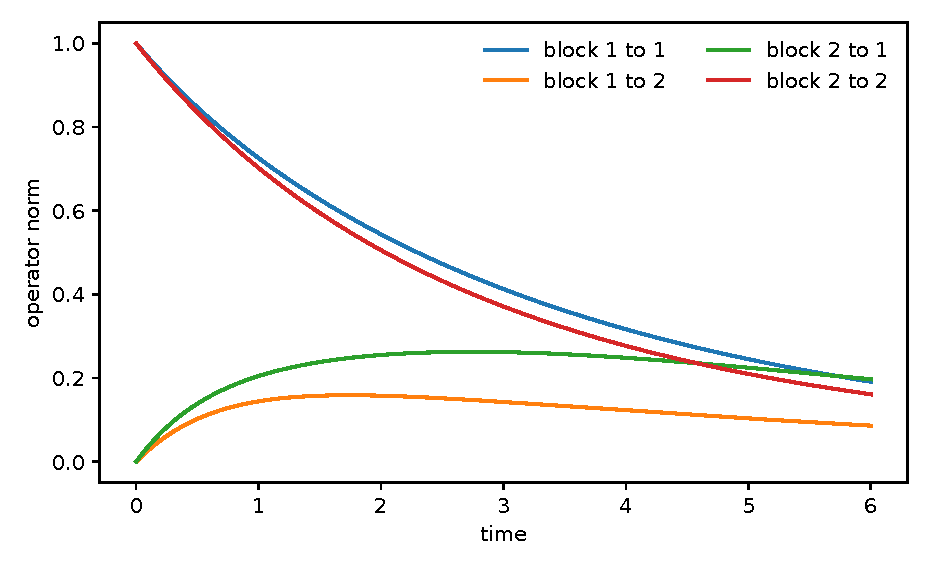
\includegraphics[width=0.72\textwidth]{packet_semigroup_blocks.pdf}
\caption{A bounded semigroup resolved into four packet blocks. The diagonal curves record persistence inside a packet. The other curves record transfer between packets.}
\label{fig:packet_semigroup_blocks}
\end{figure}

The convolution law is exact but does not show how many transfers are needed to produce a block. For that purpose, split the generator into its diagonal and off diagonal parts:
\[
D=\sum_\alpha P_\alpha AP_\alpha,
\qquad
N=A-D.
\]
Write
\[
D_\alpha=P_\alpha AP_\alpha,
\qquad
N_{\beta\alpha}=P_\beta AP_\alpha
\quad(\beta\neq\alpha).
\]

\begin{theorem}[Time ordered packet path expansion]\label{thm:dyson_packet_paths}
Let \(A=D+N\) be bounded. Then
\[
\e^{tA}
=
\sum_{m=0}^{\infty}
\int_{0<r_1<\cdots<r_m<t}
\e^{(t-r_m)D}N\e^{(r_m-r_{m-1})D}
\cdots
N\e^{r_1D}
\dd r_1\cdots\dd r_m,
\]
where the term for \(m=0\) is \(\e^{tD}\). The series converges absolutely in operator norm, uniformly for \(t\) in bounded intervals.

For packets \(\alpha_0,\alpha_m\), the block \(P_{\alpha_m}\e^{tA}P_{\alpha_0}\) is the sum over all packet paths
\[
\alpha_0\longrightarrow\alpha_1\longrightarrow\cdots\longrightarrow\alpha_m
\]
of the integrals
\[
\begin{aligned}
\int_{0<r_1<\cdots<r_m<t}
&\e^{(t-r_m)D_{\alpha_m}}
N_{\alpha_m\alpha_{m-1}}
\e^{(r_m-r_{m-1})D_{\alpha_{m-1}}}
\cdots\\
&\qquad\cdots
N_{\alpha_1\alpha_0}
\e^{r_1D_{\alpha_0}}
\dd r_1\cdots\dd r_m.
\end{aligned}
\]
\end{theorem}

\begin{proof}
Set
\[
U(t)=\e^{-tD}\e^{tA}.
\]
Then
\[
U'(t)=\e^{-tD}N\e^{tD}U(t),
\qquad
U(0)=I.
\]
Picard iteration gives the time ordered series for \(U(t)\). Multiplication by \(\e^{tD}\) gives the displayed formula for \(\e^{tA}\). If \(0\leq t\leq T\), the norm of the term with \(m\) transfers is bounded by
\[
\e^{T\norm D}
\frac{(T\norm N)^m}{m!}.
\]
The majorant is summable, which proves absolute and locally uniform convergence.

Insert packet identities between every factor. The diagonal semigroup preserves each packet, while every factor \(N\) changes the packet according to one off diagonal block. Collecting the surviving terms gives the packet path formula.
\end{proof}

\begin{corollary}[Minimum transfer order]\label{cor:minimum_transfer_order}
Suppose every directed packet path from \(\alpha\) to \(\beta\) uses at least \(m_0\) off diagonal transfers. Then
\[
P_\beta\e^{tA}P_\alpha
=O(t^{m_0})
\quad\text{as }t\downarrow0.
\]
If there is no directed path from \(\alpha\) to \(\beta\), the block vanishes for all \(t\).
\end{corollary}

\begin{proof}
Every nonzero term in \cref{thm:dyson_packet_paths} contains at least \(m_0\) time integrations. The simplex \(0<r_1<\cdots<r_m<t\) has volume \(t^m/m!\), so the first possible order is \(t^{m_0}\). If there is no path, every packet term vanishes.
\end{proof}


\begin{example}[One transfer between two packets]\label{ex:two_packet_transfer}
Let
\[
A=
\begin{pmatrix}
a&0\\
c&b
\end{pmatrix}
\]
and let the two coordinate axes be the packet spaces. If \(a\neq b\), then
\[
\e^{tA}
=
\begin{pmatrix}
\e^{at}&0\\
\displaystyle c\frac{\e^{at}-\e^{bt}}{a-b}&\e^{bt}
\end{pmatrix}.
\]
The lower left block is produced by one transfer from the first packet to the second. Its expansion begins with \(ct\), in agreement with \cref{cor:minimum_transfer_order}. When \(a=b\), the same block is \(ct\e^{at}\).
\end{example}

\begin{proposition}[Block differential equation]\label{prop:block_differential_equation}
If \(A\) is bounded, then
\[
\frac{\dd}{\dd t}T_{\beta\alpha}(t)
=
\sum_\gamma A_{\beta\gamma}T_{\gamma\alpha}(t)
=
\sum_\gamma T_{\beta\gamma}(t)A_{\gamma\alpha}.
\]
The initial condition is
\[
T_{\beta\alpha}(0)=\delta_{\beta\alpha}P_\alpha.
\]
\end{proposition}

\begin{proof}
Differentiate \(P_\beta\e^{tA}P_\alpha\) and insert the packet identity between \(A\) and the semigroup. The second equality follows from \(A\e^{tA}=\e^{tA}A\).
\end{proof}

\begin{proposition}[Packet resolvent convolution]\label{prop:packet_resolvent}
Let \(z\) belong to the resolvent set of \(A\). If \(\operatorname{Re}z\) is larger than a growth bound for the semigroup, then
\[
P_\beta(zI-A)^{-1}P_\alpha
=
\int_0^{\infty}\e^{-zt}T_{\beta\alpha}(t)\dd t.
\]
\end{proposition}

\begin{proof}
The standard Laplace representation of the resolvent is
\[
(zI-A)^{-1}
=
\int_0^{\infty}\e^{-zt}T(t)\dd t.
\]
Multiplication by the bounded packet projections may be passed through the Bochner integral.
\end{proof}

\begin{remark}
The packet path formula does not assert that the decomposition is sparse. Sparsity comes from vanishing transfer blocks or from additional smallness estimates. The formula records the exact terms that must be controlled once such structure is present.
\end{remark}

\section{Refinement defects and projective limits}\label{sec:refinement}

Let \(X_f\) and \(X_c\) be Banach spaces. Let \((T_f(t))\) and \((T_c(t))\) be strongly continuous semigroups with generators \(A_f\) and \(A_c\). For the first results, assume that both generators are bounded. Let
\[
C:X_f\longrightarrow X_c
\]
be bounded and define the generator defect
\[
\Delta=CA_f-A_cC.
\]

\begin{theorem}[Duhamel refinement identity]\label{thm:duhamel_refinement}
For every \(t\geq0\),
\[
\boxed{
CT_f(t)-T_c(t)C
=
\int_0^tT_c(t-r)\Delta T_f(r)\dd r.
}
\]
In particular, \(\Delta=0\) implies exact semigroup intertwining.
\end{theorem}

\begin{proof}
For fixed \(t\), define
\[
F(r)=T_c(t-r)CT_f(r).
\]
The bounded generator hypothesis gives
\[
F'(r)=T_c(t-r)(CA_f-A_cC)T_f(r).
\]
Integrating from \(0\) to \(t\) gives the result.
\end{proof}

\begin{corollary}[Duhamel norm bound]\label{cor:duhamel_bound}
Suppose
\[
\norm{T_f(t)}\leq M_f\e^{\omega_f t},
\qquad
\norm{T_c(t)}\leq M_c\e^{\omega_c t}.
\]
Then
\[
\norm{CT_f(t)-T_c(t)C}
\leq
M_fM_c\norm\Delta
\int_0^t\e^{\omega_c(t-r)+\omega_f r}\dd r.
\]
If both semigroups are contractions, then
\[
\norm{CT_f(t)-T_c(t)C}
\leq t\norm\Delta.
\]
\end{corollary}

\begin{proof}
Take norms in \cref{thm:duhamel_refinement} and apply the two growth bounds.
\end{proof}

\begin{figure}
\centering
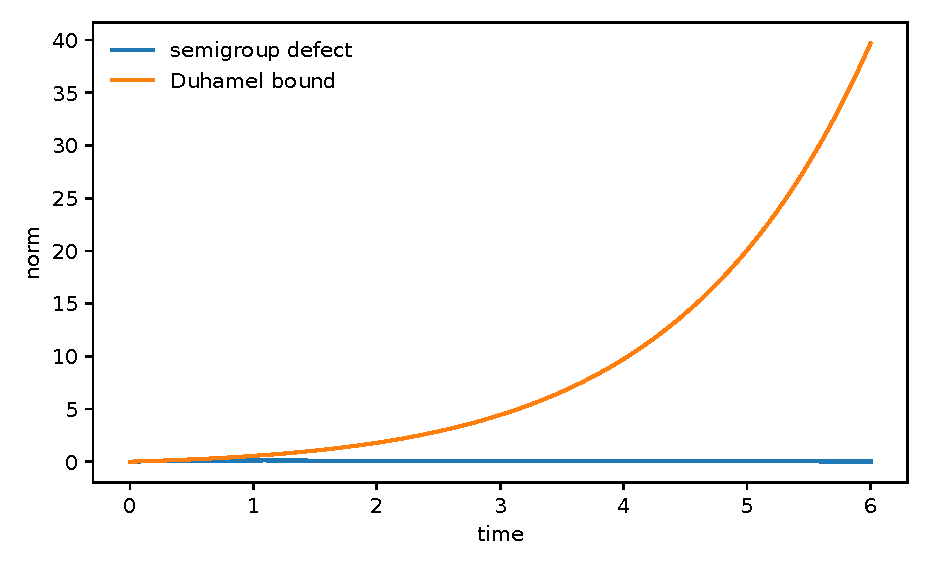
\includegraphics[width=0.72\textwidth]{refinement_defect.pdf}
\caption{A semigroup defect and a direct Duhamel bound produced by the generator defect. The bound is not expected to be sharp for every time.}
\label{fig:refinement_defect}
\end{figure}

\begin{theorem}[Resolvent refinement identity]\label{thm:resolvent_refinement}
Let \(z\) belong to the resolvent sets of \(A_f\) and \(A_c\). Then
\[
\boxed{
C(zI-A_f)^{-1}-(zI-A_c)^{-1}C
=
(zI-A_c)^{-1}\Delta(zI-A_f)^{-1}.
}
\]
\end{theorem}

\begin{proof}
Multiply the left side by \(zI-A_c\) on the left and \(zI-A_f\) on the right. The result is
\[
(zI-A_c)C-C(zI-A_f)=CA_f-A_cC=\Delta.
\]
Multiplication by the two resolvents gives the formula.
\end{proof}

\begin{corollary}[Holomorphic functional defect]\label{cor:holomorphic_defect}
Let \(\Gamma\) be a positively oriented contour surrounding both spectra. If \(F\) is holomorphic inside \(\Gamma\), then
\[
CF(A_f)-F(A_c)C
=
\frac{1}{2\pi\ii}
\int_\Gamma
F(z)(zI-A_c)^{-1}\Delta(zI-A_f)^{-1}\dd z.
\]
Consequently,
\[
\begin{aligned}
\norm{CF(A_f)-F(A_c)C}
\leq{}&
\frac{\operatorname{length}(\Gamma)}{2\pi}
\sup_{z\in\Gamma}\abs{F(z)}\norm\Delta\\
&\times
\sup_{z\in\Gamma}\norm{(zI-A_c)^{-1}}
\sup_{z\in\Gamma}\norm{(zI-A_f)^{-1}}.
\end{aligned}
\]
\end{corollary}

\begin{proof}
Apply the Cauchy integral formula for matrix or bounded operator functions and insert \cref{thm:resolvent_refinement}.
\end{proof}

We next pass to several levels. For integers \(\ell<m\), let
\[
C_{\ell,m}=C_\ell C_{\ell+1}\cdots C_{m-1},
\qquad
C_{\ell,\ell}=I,
\]
where \(C_j:X_{j+1}\to X_j\).

\begin{theorem}[Several level telescoping identity]\label{thm:multilevel_telescoping}
Let \(T_j\) be bounded operators on \(X_j\), and set
\[
E_j=C_jT_{j+1}-T_jC_j.
\]
Then
\[
\boxed{
C_{\ell,m}T_m-T_\ell C_{\ell,m}
=
\sum_{j=\ell}^{m-1}
C_{\ell,j}E_jC_{j+1,m}.
}
\]
\end{theorem}

\begin{proof}
Expand each summand as
\[
C_{\ell,j+1}T_{j+1}C_{j+1,m}
-
C_{\ell,j}T_jC_{j,m}.
\]
The intermediate terms cancel. The first surviving term is \(C_{\ell,m}T_m\), and the last is \(-T_\ell C_{\ell,m}\).
\end{proof}

\begin{corollary}[Summable generator defects]\label{cor:summable_defects}
Suppose \(C_j\) are contractions and \((T_j(t))\) are contraction semigroups with bounded generators \(A_j\). Set
\[
\delta_j=\norm{C_jA_{j+1}-A_jC_j}.
\]
Then
\[
\norm{C_{\ell,m}T_m(t)-T_\ell(t)C_{\ell,m}}
\leq
 t\sum_{j=\ell}^{m-1}\delta_j.
\]
If \(\sum_{j\geq0}\delta_j<\infty\), the right side tends to zero as \(\ell\to\infty\), uniformly in \(m>\ell\) and uniformly for \(t\) in a fixed bounded interval.
\end{corollary}

\begin{proof}
By \cref{cor:duhamel_bound}, the interlevel semigroup defect has norm at most \(t\delta_j\). Apply \cref{thm:multilevel_telescoping} and use the contraction bounds on all coarsening maps.
\end{proof}

\begin{definition}[Projective limit space]\label{def:projective_limit}
Let \((X_j,C_j)\) be a sequence of Banach spaces and continuous maps \(C_j:X_{j+1}\to X_j\). Its projective limit is
\[
X_\infty
=
\left\{
(x_j)_{j\geq0}\in\prod_{j\geq0}X_j:
C_jx_{j+1}=x_j\text{ for every }j
\right\}.
\]
We equip \(X_\infty\) with the subspace topology inherited from the product topology.
\end{definition}

\begin{theorem}[Exact projective limit semigroup]\label{thm:projective_limit_semigroup}
Suppose each \(X_j\) carries a strongly continuous semigroup \((T_j(t))_{t\geq0}\), and
\[
C_jT_{j+1}(t)=T_j(t)C_j
\]
for every \(j\) and every \(t\geq0\). Then
\[
T_\infty(t)(x_j)_{j\geq0}
=
(T_j(t)x_j)_{j\geq0}
\]
defines a strongly continuous semigroup on \(X_\infty\).
\end{theorem}

\begin{proof}
Exact intertwining gives
\[
C_jT_{j+1}(t)x_{j+1}
=
T_j(t)C_jx_{j+1}
=
T_j(t)x_j.
\]
Thus the coordinatewise evolution remains in the projective limit. The semigroup law holds in every coordinate. Strong continuity in the product topology follows because every coordinate map
\[
t\longmapsto T_j(t)x_j
\]
is continuous.
\end{proof}

\begin{corollary}[Coordinate generators]\label{cor:projective_generators}
Assume the setting of \cref{thm:projective_limit_semigroup}. If \(x=(x_j)\) satisfies \(x_j\in\operatorname{Dom}(A_j)\) and the sequence \((A_jx_j)\) belongs to \(X_\infty\), then \(x\) lies in the generator domain of \(T_\infty\) and
\[
A_\infty x=(A_jx_j)_{j\geq0}.
\]
\end{corollary}

\begin{proof}
The difference quotients converge in every coordinate to \(A_jx_j\). The assumed compatibility places the coordinatewise limit in \(X_\infty\), which is exactly convergence in the product topology.
\end{proof}

\begin{figure}
\centering
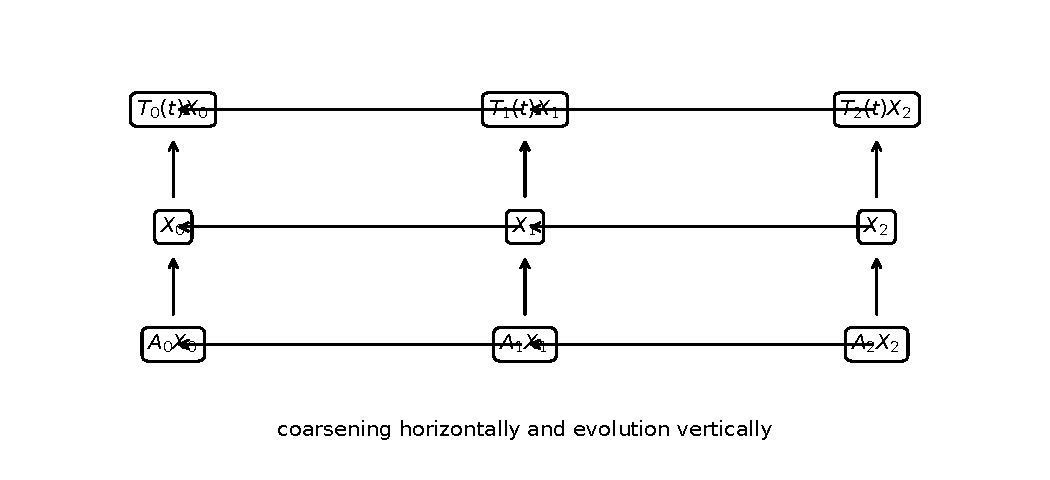
\includegraphics[width=0.82\textwidth]{projective_tower.pdf}
\caption{An exact projective tower. Coarsening commutes with the evolution and with the generator on their common domains.}
\label{fig:projective_tower}
\end{figure}

\begin{remark}
Summable defects do not by themselves define a new exact generator on \(X_\infty\). They show that fine evolutions become asymptotically compatible when observed through sufficiently deep common coarse levels. Constructing an exact limit from approximate data needs an additional convergence, compactness, or correction argument.
\end{remark}

\section{Markov semigroups and lumping}\label{sec:markov}

We use column probability vectors. A matrix \(Q\in\RR^{n\times n}\) is a Markov generator when its off diagonal entries are nonnegative and its column sums are zero. The distribution at time \(t\) is
\[
p(t)=\e^{tQ}p(0).
\]

\begin{theorem}[Finite Markov semigroup]\label{thm:finite_markov_semigroup}
If \(Q\) is a Markov generator, then \(\e^{tQ}\) has nonnegative entries and column sums one for every \(t\geq0\).
\end{theorem}

\begin{proof}
Choose \(\lambda\geq\max_i(-Q_{ii})\). The matrix \(B=Q+\lambda I\) is entrywise nonnegative. Hence \(\e^{tB}\) is entrywise nonnegative by its power series, and
\[
\e^{tQ}=\e^{-\lambda t}\e^{tB}
\]
is nonnegative. Since \(\one^TQ=0\),
\[
\frac{\dd}{\dd t}\one^T\e^{tQ}=0.
\]
At \(t=0\), this row vector is \(\one^T\), so the column sums remain one.
\end{proof}

Let \(B_1,\ldots,B_m\) be a partition of the fine state set \(\{1,\ldots,n\}\). Define the aggregation matrix \(C\in\RR^{m\times n}\) by
\[
C_{ai}=\one_{\{i\in B_a\}}.
\]
Thus \((Cp)_a\) is the total fine mass in block \(B_a\).

\begin{definition}[Strong lumpability]\label{def:strong_lumpability}
The generator \(Q\) is strongly lumpable with respect to the partition if there is a Markov generator \(\overline Q\in\RR^{m\times m}\) such that
\[
CQ=\overline QC.
\]
\end{definition}

\begin{theorem}[Aggregate rate criterion]\label{thm:aggregate_rate_criterion}
A Markov generator \(Q\) is strongly lumpable if and only if, for every pair \(i,j\in B_b\) and every coarse block \(B_a\),
\[
\boxed{
\sum_{k\in B_a}Q_{ki}
=
\sum_{k\in B_a}Q_{kj}.
}
\]
When this condition holds, the coarse generator is uniquely determined by
\[
\overline Q_{ab}
=
\sum_{k\in B_a}Q_{ki}
\quad\text{for any }i\in B_b.
\]
\end{theorem}

\begin{proof}
The \((a,i)\) entry of \(CQ\) is
\[
(CQ)_{ai}=\sum_{k\in B_a}Q_{ki}.
\]
If \(i\in B_b\), then the \(i\)th column of \(\overline QC\) is the \(b\)th column of \(\overline Q\). Therefore \(CQ=\overline QC\) is possible exactly when the displayed aggregate rate depends only on the block \(B_b\) containing \(i\). The resulting matrix has nonnegative off diagonal entries. Its column sums are zero because the column sums of \(Q\) are zero.
\end{proof}

\begin{corollary}[Exact continuous time lumping]\label{cor:exact_continuous_lumping}
If \(CQ=\overline QC\), then
\[
\boxed{
C\e^{tQ}=\e^{t\overline Q}C
}
\]
for every \(t\geq0\).
\end{corollary}

\begin{proof}
Apply \cref{thm:duhamel_refinement} with zero generator defect. Equivalently, use the equality \(CQ^r=\overline Q^rC\) in the exponential series.
\end{proof}

\begin{theorem}[Discrete horizon defect]\label{thm:discrete_lumping_defect}
Let \(K\) and \(\overline K\) be stochastic matrices and set
\[
\Delta_K=CK-\overline KC.
\]
Then
\[
\boxed{
CK^r-\overline K^rC
=
\sum_{j=0}^{r-1}
\overline K^{r-1-j}\Delta_KK^j.
}
\]
If \(K\) and \(\overline K\) are contractions in the chosen norm, then
\[
\norm{CK^r-\overline K^rC}
\leq r\norm{\Delta_K}.
\]
\end{theorem}

\begin{proof}
Write each summand as
\[
\overline K^{r-1-j}CK^{j+1}
-
\overline K^{r-j}CK^j.
\]
The sum telescopes. The norm estimate follows term by term.
\end{proof}

\begin{theorem}[Continuous time lumping defect]\label{thm:continuous_lumping_defect}
For generators \(Q\) and \(\overline Q\), set
\[
\Delta_Q=CQ-\overline QC.
\]
Then
\[
C\e^{tQ}-\e^{t\overline Q}C
=
\int_0^t
\e^{(t-r)\overline Q}
\Delta_Q
\e^{rQ}
\dd r.
\]
In the probability \(\ell^1\) norm,
\[
\norm{C\e^{tQ}-\e^{t\overline Q}C}_1
\leq t\norm{\Delta_Q}_1
\]
whenever both semigroups are stochastic contractions.
\end{theorem}

\begin{proof}
This is \cref{thm:duhamel_refinement} and \cref{cor:duhamel_bound} in the Markov setting.
\end{proof}

\begin{figure}
\centering
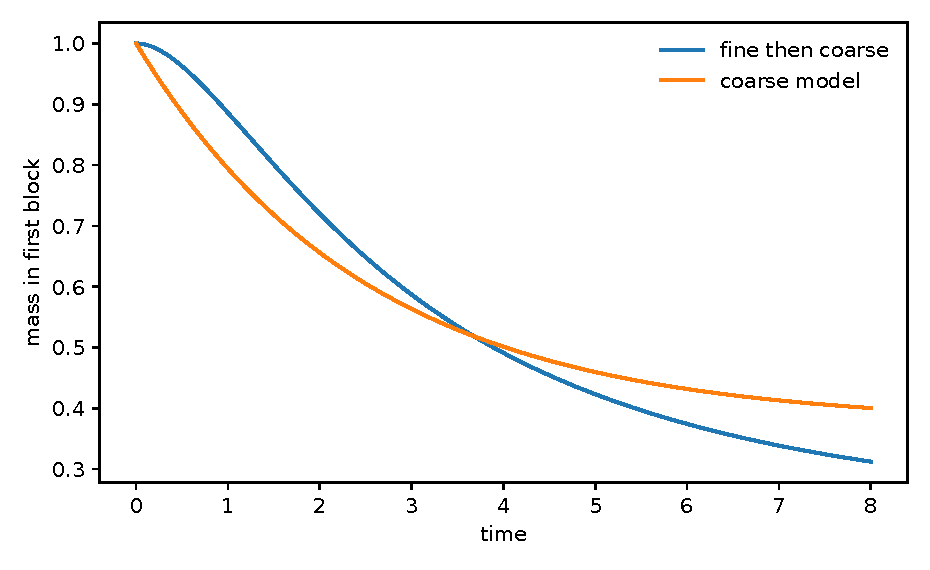
\includegraphics[width=0.72\textwidth]{markov_lumping.pdf}
\caption{Fine evolution followed by aggregation compared with a coarse Markov model. Exact lumping makes the curves coincide. A nonzero aggregate rate defect separates them.}
\label{fig:markov_lumping}
\end{figure}


\begin{example}[A four state lumpable chain]\label{ex:four_state_lumping}
Partition four states into \(B_1=\{1,2\}\) and \(B_2=\{3,4\}\). For positive rates \(a,b,u,v\), set
\[
Q=
\begin{pmatrix}
-u-a&u&b/2&b/2\\
u&-u-a&b/2&b/2\\
a/2&a/2&-v-b&v\\
a/2&a/2&v&-v-b
\end{pmatrix}.
\]
The rates \(u\) and \(v\) move inside the coarse blocks. Every state in \(B_1\) leaves for \(B_2\) at total rate \(a\), and every state in \(B_2\) leaves for \(B_1\) at total rate \(b\). Hence
\[
\overline Q=
\begin{pmatrix}
-a&b\\
a&-b
\end{pmatrix}
\]
and \(CQ=\overline QC\). The internal rates disappear from the coarse generator even though they remain present in the fine evolution.
\end{example}

\begin{theorem}[Reversibility descends]\label{thm:reversibility_descends}
Assume \(Q\) is strongly lumpable and reversible with respect to a positive stationary distribution \(\pi\), so
\[
Q_{ij}\pi_j=Q_{ji}\pi_i.
\]
Define
\[
\overline\pi_a=\sum_{i\in B_a}\pi_i.
\]
Then \(\overline\pi\) is stationary for \(\overline Q\), and
\[
\overline Q_{ab}\overline\pi_b
=
\overline Q_{ba}\overline\pi_a.
\]
Thus the coarse chain is reversible.
\end{theorem}

\begin{proof}
Stationarity follows from
\[
\overline Q\overline\pi
=\overline QC\pi
=CQ\pi=0.
\]
For reversibility, use the aggregate rate formula:
\[
\begin{aligned}
\overline Q_{ab}\overline\pi_b
&=\sum_{j\in B_b}\pi_j\sum_{i\in B_a}Q_{ij}\\
&=\sum_{i\in B_a}\sum_{j\in B_b}\pi_iQ_{ji}\\
&=\overline Q_{ba}\overline\pi_a.
\end{aligned}
\]
\end{proof}

\begin{corollary}[Coarse Dirichlet form]\label{cor:coarse_dirichlet_form}
Under the hypotheses of \cref{thm:reversibility_descends}, let \(Jg\) be the fine function that is constant with value \(g_a\) on \(B_a\). Then
\[
-\ip{Jg}{Q^TJg}_{L^2(\pi)}
=
-\ip{g}{\overline Q^Tg}_{L^2(\overline\pi)}.
\]
\end{corollary}

\begin{proof}
Expand the left side and group the fine indices by their coarse blocks. The aggregate rate criterion converts the resulting sums into the coarse generator entries.
\end{proof}

\begin{remark}
Strong lumpability is a statement about every initial distribution. Weaker notions may preserve the Markov property only for a restricted class of initial laws. Those notions are important, but they are not used in the exact intertwining results here.
\end{remark}

\section{Conditional expectation and martingale packets}\label{sec:conditional}

Let \(\Omega=\{1,\ldots,n\}\) carry positive weights \(\pi_i\) with \(\sum_i\pi_i=1\). Equip \(\RR^n\) with
\[
\ip{f}{g}_\pi
=
\sum_{i=1}^n\pi_if_ig_i.
\]
For a partition \(\Qcal=\{B_1,\ldots,B_m\}\), define
\[
(P_\Qcal f)_i
=
\frac{\sum_{j\in B(i)}\pi_jf_j}
{\sum_{j\in B(i)}\pi_j}.
\]

\begin{theorem}[Finite conditional expectation]\label{thm:finite_conditional_expectation}
The operator \(P_\Qcal\) is the orthogonal projection in \(L^2(\pi)\) onto the subspace of functions that are constant on every block of \(\Qcal\). In particular,
\[
P_\Qcal^2=P_\Qcal,
\qquad
P_\Qcal^*=P_\Qcal.
\]
\end{theorem}

\begin{proof}
The output is block constant. If \(g\) is block constant, then on each block \(B\),
\[
\sum_{i\in B}\pi_i(f_i-(P_\Qcal f)_i)g_i
=g_B\left(
\sum_{i\in B}\pi_if_i
-(P_\Qcal f)_B\sum_{i\in B}\pi_i
\right)=0.
\]
Thus \(f-P_\Qcal f\) is orthogonal to the block constant subspace. This characterizes the orthogonal projection.
\end{proof}

\begin{theorem}[Tower law]\label{thm:tower_law}
Suppose \(\Qcal_0\) is coarser than \(\Qcal_1\). Then
\[
P_{\Qcal_0}P_{\Qcal_1}
=P_{\Qcal_0}
=P_{\Qcal_1}P_{\Qcal_0}.
\]
\end{theorem}

\begin{proof}
The range of \(P_{\Qcal_0}\) is contained in the range of \(P_{\Qcal_1}\). Orthogonal projections onto nested subspaces satisfy the displayed identities. The same conclusion follows directly by averaging the fine block averages over each coarse block.
\end{proof}

Let
\[
\Qcal_0\preceq\Qcal_1\preceq\cdots\preceq\Qcal_m
\]
be nested partitions, and set \(P_r=P_{\Qcal_r}\). Define
\[
D_0=P_0,
\qquad
D_r=P_r-P_{r-1}
\quad(r\geq1).
\]

\begin{theorem}[Martingale packet decomposition]\label{thm:martingale_packets}
The operators \(D_0,\ldots,D_m\) are pairwise orthogonal projections and
\[
P_m=\sum_{r=0}^mD_r.
\]
For every \(f\),
\[
\boxed{
\norm{P_mf}_{L^2(\pi)}^2
=
\sum_{r=0}^m\norm{D_rf}_{L^2(\pi)}^2.
}
\]
If \(P_m=I\), then the same formula holds with \(f\) on the left.
\end{theorem}

\begin{proof}
The tower law gives
\[
D_r^2=(P_r-P_{r-1})^2=P_r-P_{r-1}=D_r.
\]
Each \(D_r\) is self adjoint. If \(r<s\), then
\[
D_rD_s
=(P_r-P_{r-1})(P_s-P_{s-1})=0
\]
by the tower law. The sum telescopes to \(P_m\). The norm identity is the Pythagorean theorem.
\end{proof}

\begin{corollary}[Variance decomposition]\label{cor:variance_decomposition}
If \(P_0f=\EE_\pi[f]\one\) and \(P_m=I\), then
\[
\Var_\pi(f)
=
\sum_{r=1}^m\norm{D_rf}_{L^2(\pi)}^2.
\]
\end{corollary}

\begin{proof}
Apply \cref{thm:martingale_packets} and remove the squared norm of the constant mean packet.
\end{proof}

\begin{figure}
\centering
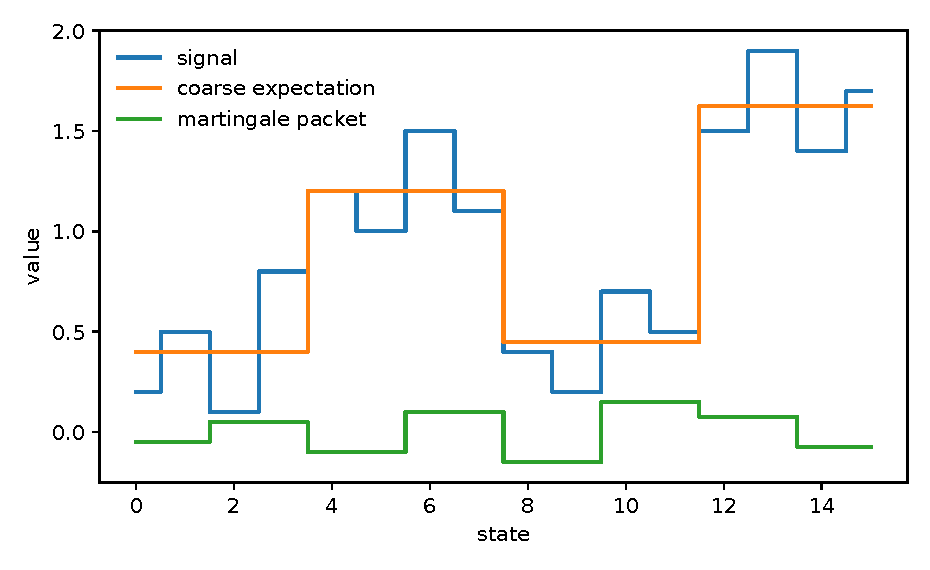
\includegraphics[width=0.72\textwidth]{martingale_packets.pdf}
\caption{A finite signal, its coarse conditional expectation, and one martingale packet. The packet has zero weighted mean on every coarse block.}
\label{fig:martingale_packets}
\end{figure}

\begin{proposition}[Conditional variance identity]\label{prop:conditional_variance}
For any partition \(\Qcal\),
\[
\norm{f-P_\Qcal f}_{L^2(\pi)}^2
=
\sum_{B\in\Qcal}
\sum_{i\in B}\pi_i
\left(f_i-\EE_\pi[f\mid B]\right)^2.
\]
This quantity is the total within block variance.
\end{proposition}

\begin{proof}
The identity is the definition of the weighted norm after writing the projection as the block conditional mean.
\end{proof}

\section{Bayesian transfer and sufficiency}\label{sec:bayes}

Let
\[
\Delta_n
=
\left\{p\in\RR^n:p_i\geq0,\ \sum_i p_i=1\right\}
\]
be the probability simplex. A positive likelihood is a vector \(L\in(0,\infty)^n\). Define the Bayesian transfer
\[
\Bcal_L(p)
=
\frac{L\odot p}{\ip{L}{p}},
\]
where \(\odot\) denotes coordinatewise multiplication.

\begin{proposition}[Independent likelihood composition]\label{prop:bayes_composition}
For positive likelihoods \(L\) and \(M\),
\[
\boxed{
\Bcal_M\bigl(\Bcal_L(p)\bigr)
=
\Bcal_{M\odot L}(p).
}
\]
Likelihood multiplication is therefore transported to composition of normalized Bayesian maps.
\end{proposition}

\begin{proof}
The numerator after two updates is \(M\odot L\odot p\). The first evidence appears in both the numerator and denominator of the second update and cancels.
\end{proof}

Let \(B_1,\ldots,B_m\) be a partition of the state set and let \(C\) be its mass aggregation map. Define the packet evidence
\[
Z_a(p,L)=\sum_{i\in B_a}L_ip_i,
\qquad
Z(p,L)=\sum_aZ_a(p,L).
\]
When \(Z_a>0\), define the conditional posterior packet
\[
r_i^{(a)}
=
\frac{L_ip_i}{Z_a}
\quad(i\in B_a),
\]
and set it to zero outside \(B_a\).

\begin{theorem}[Packet evidence reconstruction]\label{thm:packet_evidence}
The posterior has the exact decomposition
\[
\boxed{
\Bcal_L(p)
=
\sum_{a=1}^m
\frac{Z_a(p,L)}{Z(p,L)}r^{(a)}.
}
\]
Its coarse mass vector is
\[
C\Bcal_L(p)
=
\left(
\frac{Z_a(p,L)}{Z(p,L)}
\right)_{a=1}^m.
\]
\end{theorem}

\begin{proof}
For \(i\in B_a\), the \(i\)th coordinate of the right side is
\[
\frac{Z_a}{Z}\frac{L_ip_i}{Z_a}
=
\frac{L_ip_i}{Z}.
\]
Summing the posterior coordinates inside each block gives the coarse mass formula.
\end{proof}

For a coarse likelihood \(\overline L\in(0,\infty)^m\), define
\[
\Bcal_{\overline L}(q)
=
\frac{\overline L\odot q}{\ip{\overline L}{q}}.
\]

\begin{theorem}[Finite Bayesian sufficiency criterion]\label{thm:bayesian_sufficiency}
Assume the partition has at least two nonempty blocks. The following statements are equivalent.

\begin{enumerate}
\item There is a positive coarse likelihood \(\overline L\) such that
\[
C\Bcal_L(p)
=
\Bcal_{\overline L}(Cp)
\]
for every prior \(p\in\Delta_n\).

\item The likelihood \(L\) is constant inside every block.
\end{enumerate}

When these conditions hold, \(\overline L_a\) may be chosen to equal the common value of \(L\) on \(B_a\). Any other coarse likelihood giving the same update for every prior differs by one positive scalar factor.
\end{theorem}

\begin{proof}
If \(L_i=\ell_a\) on \(B_a\), then
\[
Z_a=\ell_a(Cp)_a.
\]
The packet evidence formula gives exact commutation with \(\overline L=(\ell_a)\).

Conversely, choose distinct blocks \(B_a\) and \(B_b\), a state \(i\in B_a\), and a state \(k\in B_b\). Apply the assumed identity to priors supported on \(i\) and \(k\), with arbitrary positive masses \(u\) and \(v\). Equality of the posterior mass in block \(B_a\) gives
\[
\frac{L_iu}{L_iu+L_kv}
=
\frac{\overline L_au}{\overline L_au+\overline L_bv}.
\]
Hence
\[
\frac{L_i}{L_k}
=
\frac{\overline L_a}{\overline L_b}.
\]
Replacing \(i\) by any other state in \(B_a\) shows that \(L\) is constant on \(B_a\). Repeating the argument for every block proves the claim. The same ratio identity shows uniqueness of \(\overline L\) up to a common positive factor.
\end{proof}

\begin{remark}
For a partition with one block, the coarse posterior is always the single point mass. No within block likelihood information can be detected at that level. The nontrivial criterion begins when at least two coarse blocks can compete for posterior mass.
\end{remark}

A weaker exact statement is available for a restricted prior family. Fix probability vectors \(r^{(a)}\) supported on \(B_a\). Consider priors of the form
\[
p_i=q_ar_i^{(a)}
\quad(i\in B_a),
\qquad
q\in\Delta_m.
\]

\begin{proposition}[Sufficiency relative to a prior disintegration]\label{prop:relative_sufficiency}
Define
\[
\overline L_a
=
\sum_{i\in B_a}L_ir_i^{(a)}.
\]
For every prior in the declared family,
\[
C\Bcal_L(p)
=
\Bcal_{\overline L}(q).
\]
\end{proposition}

\begin{proof}
The evidence in block \(B_a\) is
\[
Z_a
=q_a\sum_{i\in B_a}L_ir_i^{(a)}
=q_a\overline L_a.
\]
Apply \cref{thm:packet_evidence}.
\end{proof}

\begin{lemma}[Normalization bound]\label{lem:normalization_bound}
Let \(a,b\in[0,\infty)^m\) be nonzero, and set \(A=\norm a_1\) and \(B=\norm b_1\). Then
\[
\boxed{
\norm{a/A-b/B}_1
\leq
\frac{2\norm{a-b}_1}{\max\{A,B\}}.
}
\]
\end{lemma}

\begin{proof}
Using \(A\) in the denominator gives
\[
\norm{a/A-b/B}_1
\leq
\frac{\norm{a-b}_1}{A}
+
\norm b_1\abs{1/A-1/B}.
\]
The second term equals \(\abs{B-A}/A\), which is at most \(\norm{a-b}_1/A\). Interchanging \(a\) and \(b\) gives the analogous bound with \(B\). Taking the smaller of the two bounds gives the result.
\end{proof}

For a prior \(p\), write \(q=Cp\). When \(q_a>0\), define the exact coarse likelihood
\[
\ell_a(p)
=
\frac{\sum_{i\in B_a}L_ip_i}{q_a}.
\]
If \(q_a=0\), its value is irrelevant.

\begin{theorem}[Exact information loss formula]\label{thm:information_loss}
For every prior,
\[
\boxed{
C\Bcal_L(p)
=
\Bcal_{\ell(p)}(q).
}
\]
Let \(\overline L\) be any fixed positive coarse likelihood and set
\[
d(p\mid L,\overline L)
=
\sum_{a=1}^mq_a\abs{\ell_a(p)-\overline L_a}.
\]
Then
\[
\norm{
C\Bcal_L(p)-\Bcal_{\overline L}(q)
}_1
\leq
\frac{2d(p\mid L,\overline L)}
{\max\{Z(p,L),\ip{\overline L}{q}\}}.
\]
\end{theorem}

\begin{proof}
The packet evidence in block \(a\) is \(q_a\ell_a(p)\), which proves the exact identity. Apply \cref{lem:normalization_bound} to
\[
a=q\odot\ell(p),
\qquad
b=q\odot\overline L.
\]
Their \(\ell^1\) norms are the two evidences, and \(\norm{a-b}_1=d(p\mid L,\overline L)\).
\end{proof}

\begin{corollary}[Oscillation bound]\label{cor:bayes_oscillation}
Suppose \(\overline L_a\) is any representative likelihood for block \(B_a\), and set
\[
\omega_a
=
\max_{i\in B_a}\abs{L_i-\overline L_a}.
\]
Then
\[
d(p\mid L,\overline L)
\leq
\sum_aq_a\omega_a.
\]
Thus small within block likelihood oscillation gives a small coarse posterior defect whenever the evidence is bounded away from zero.
\end{corollary}

\begin{proof}
The conditional average \(\ell_a(p)\) lies in the convex hull of the likelihood values inside \(B_a\). Hence
\[
\abs{\ell_a(p)-\overline L_a}\leq\omega_a.
\]
Multiply by \(q_a\) and sum.
\end{proof}


\begin{example}[A visible likelihood loss]\label{ex:bayes_information_loss}
Let \(B_1=\{1,2\}\), let \(B_2=\{3\}\), and take
\[
p=(3/10,2/10,5/10),
\qquad
L=(1,3,2).
\]
The coarse prior is \((1/2,1/2)\). The exact block likelihoods are
\[
\ell_1(p)=\frac{(3/10)+3(2/10)}{1/2}=\frac95,
\qquad
\ell_2(p)=2.
\]
Thus the exact coarse posterior is \((9/19,10/19)\). If the first block is replaced by the fixed representative value \(2\), the approximate coarse posterior is \((1/2,1/2)\). The \(\ell^1\) defect is \(1/19\), while \cref{thm:information_loss} gives the valid upper bound \(1/10\).
\end{example}

\begin{figure}
\centering
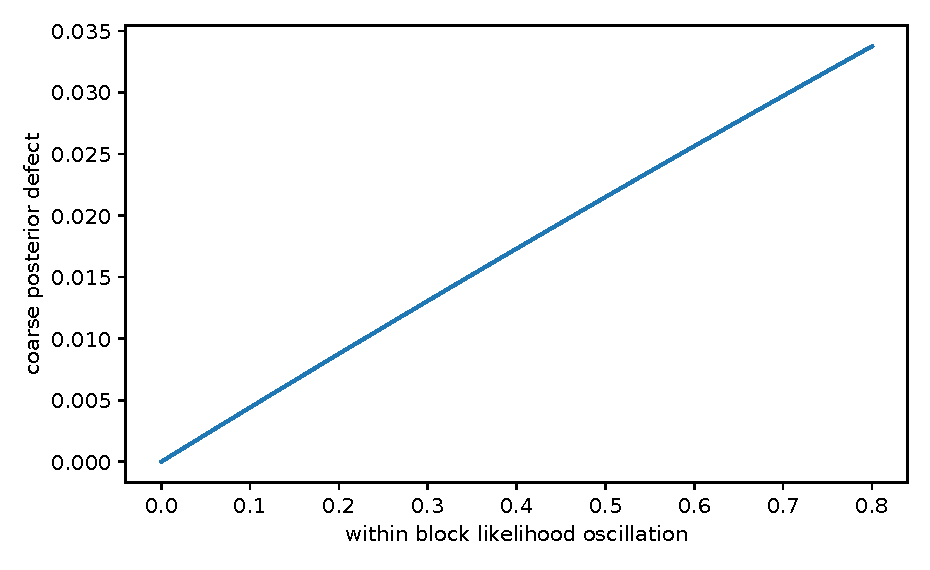
\includegraphics[width=0.72\textwidth]{bayesian_sufficiency.pdf}
\caption{A coarse posterior defect produced by likelihood variation inside one block. The defect vanishes when the likelihood is block constant.}
\label{fig:bayesian_sufficiency}
\end{figure}

\begin{proposition}[Stability with respect to the prior]\label{prop:bayes_prior_stability}
Assume
\[
0<m\leq L_i\leq M
\]
for all \(i\). Then
\[
\norm{\Bcal_L(p)-\Bcal_L(q)}_1
\leq
\frac{2M}{m}\norm{p-q}_1.
\]
\end{proposition}

\begin{proof}
Apply \cref{lem:normalization_bound} to \(a=L\odot p\) and \(b=L\odot q\). Their evidences are at least \(m\), and
\[
\norm{a-b}_1\leq M\norm{p-q}_1.
\]
\end{proof}

\begin{proposition}[Stability with respect to the likelihood]\label{prop:bayes_likelihood_stability}
For positive likelihoods \(L\) and \(M\),
\[
\norm{\Bcal_L(p)-\Bcal_M(p)}_1
\leq
\frac{2\sum_i p_i\abs{L_i-M_i}}
{\max\{\ip{L}{p},\ip{M}{p}\}}.
\]
\end{proposition}

\begin{proof}
Apply \cref{lem:normalization_bound} to \(L\odot p\) and \(M\odot p\).
\end{proof}

\subsection{Bayesian flows}\label{sec:bayesian_flows}

For a score vector \(g\in\RR^n\), define
\[
\Bcal_t^g(p)_i
=
\frac{\e^{tg_i}p_i}{\sum_j\e^{tg_j}p_j}.
\]

\begin{theorem}[Bayesian nonlinear semigroup]\label{thm:bayesian_flow}
The maps \((\Bcal_t^g)_{t\geq0}\) satisfy
\[
\Bcal_s^g\circ\Bcal_t^g
=
\Bcal_{s+t}^g.
\]
Their trajectories solve the replicator equation
\[
\boxed{
\dot p_i(t)
=
\left(g_i-\sum_jg_jp_j(t)\right)p_i(t).
}
\]
\end{theorem}

\begin{proof}
The semigroup law follows from \cref{prop:bayes_composition} because \(\e^{sg}\odot\e^{tg}=\e^{(s+t)g}\). Differentiate the explicit formula. The derivative of the normalizing denominator contributes the mean score \(\sum_jg_jp_j(t)\).
\end{proof}

\begin{corollary}[Covariance identity]\label{cor:bayesian_covariance}
For any observable \(h\in\RR^n\),
\[
\frac{\dd}{\dd t}\EE_{p(t)}[h]
=
\Cov_{p(t)}(h,g).
\]
In particular,
\[
\frac{\dd}{\dd t}\EE_{p(t)}[g]
=
\Var_{p(t)}(g)\geq0.
\]
\end{corollary}

\begin{proof}
Differentiate \(\sum_ih_ip_i(t)\) and insert the replicator equation.
\end{proof}

\begin{corollary}[Asymptotic concentration]\label{cor:bayesian_concentration}
Let \(g_*=\max_i g_i\). If the prior gives positive mass to at least one maximizing state, then
\[
\sum_{i:g_i=g_*}\Bcal_t^g(p)_i
\longrightarrow1
\quad\text{as }t\to\infty.
\]
\end{corollary}

\begin{proof}
Divide numerator and denominator by \(\e^{tg_*}\). Every term with \(g_i<g_*\) tends to zero exponentially.
\end{proof}

\begin{figure}
\centering
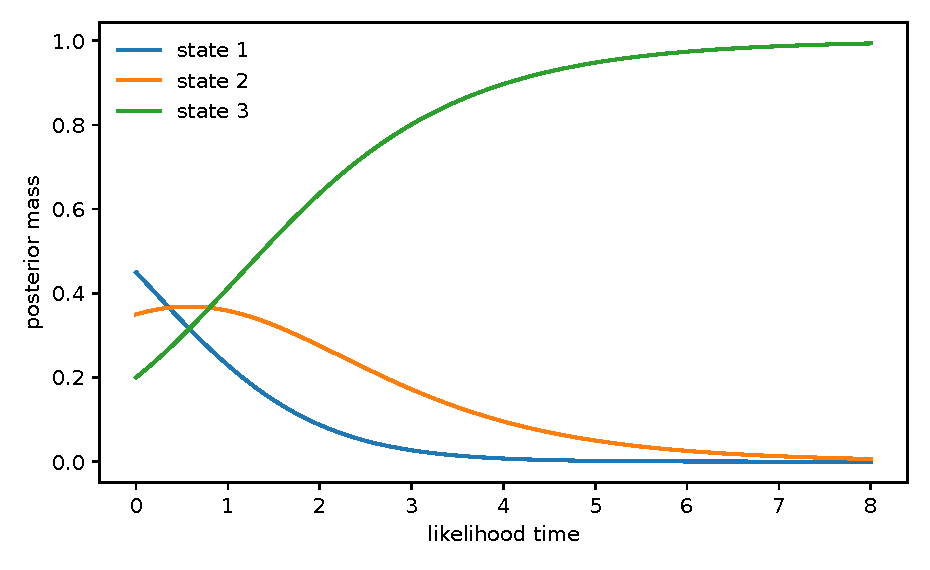
\includegraphics[width=0.72\textwidth]{bayesian_flow.pdf}
\caption{A Bayesian likelihood flow on three states. The posterior moves toward the state with the largest score while preserving the simplex.}
\label{fig:bayesian_flow}
\end{figure}

\section{Filtering through coarse packets}\label{sec:filtering}

Let \(K\) be a fine stochastic matrix and \(L_y\) a positive observation likelihood. The filtering step is
\[
\Phi_y(p)=\Bcal_{L_y}(Kp).
\]
Let \(\overline K\) and \(\overline L_y\) define the coarse filter
\[
\overline\Phi_y(q)
=
\Bcal_{\overline L_y}(\overline Kq).
\]

\begin{theorem}[Exact coarse hidden Markov filter]\label{thm:exact_coarse_filter}
Assume
\[
CK=\overline KC
\]
and every likelihood \(L_y\) is constant on each coarse block with block values \(\overline L_y\). Then
\[
C\Phi_y(p)=\overline\Phi_y(Cp)
\]
for every prior. For any observation sequence \(y_1,\ldots,y_r\), the complete filtering recursion commutes with aggregation:
\[
C\Phi_{y_r}\circ\cdots\circ\Phi_{y_1}
=
\overline\Phi_{y_r}\circ\cdots\circ\overline\Phi_{y_1}C.
\]
\end{theorem}

\begin{proof}
Exact Markov lumping gives \(CKp=\overline KCp\). The Bayesian sufficiency criterion gives exact commutation of the update. Their composition proves the one step identity. Iterate it over the observation sequence.
\end{proof}

\begin{theorem}[One step filter defect]\label{thm:filter_defect}
Let \(r=Kp\), \(q=Cr\), and let \(\ell_y(r)\) be the exact coarse likelihood obtained by averaging \(L_y\) inside each block with respect to \(r\). Assume
\[
0<\overline m\leq(\overline L_y)_a\leq\overline M.
\]
Then
\[
\begin{aligned}
\norm{C\Phi_y(p)-\overline\Phi_y(Cp)}_1
\leq{}&
\frac{2d(r\mid L_y,\overline L_y)}
{\max\{\ip{L_y}{r},\ip{\overline L_y}{q}\}}\\
&+
\frac{2\overline M}{\overline m}
\norm{CKp-\overline KCp}_1.
\end{aligned}
\]
\end{theorem}

\begin{proof}
Insert the intermediate posterior \(\Bcal_{\overline L_y}(CKp)\). The first difference is bounded by \cref{thm:information_loss}. The second is bounded by \cref{prop:bayes_prior_stability} applied to the coarse likelihood.
\end{proof}

\begin{remark}
The two terms have different meanings. The first measures observation information discarded inside coarse blocks. The second measures dynamical mass transfer that the coarse Markov model fails to reproduce.
\end{remark}

\section{Fractional powers and spectral refinement}\label{sec:fractional}

Let \(H_f\) and \(H_c\) be finite dimensional Hilbert spaces. The finite dimensional setting keeps the spectral formulas transparent and is sufficient for the refinement estimates below. The same identities extend to bounded positive self adjoint operators whenever the stated integrals converge in operator norm.

\begin{definition}[Spectral fractional power]\label{def:spectral_fractional_power}
Let \(L\) be positive and self adjoint, with spectral resolution
\[
L=\sum_{j=1}^{r}\lambda_jP_j.
\]
For \(\alpha>0\), define
\[
L^\alpha=\sum_{j=1}^{r}\lambda_j^\alpha P_j.
\]
If \(\lambda_j=0\), we use \(0^\alpha=0\).
\end{definition}

\begin{proposition}[Spectral packets]\label{prop:spectral_packets}
For every bounded scalar function \(f\) on \(\Spec L\),
\[
f(L)=\sum_{j=1}^{r}f(\lambda_j)P_j.
\]
In particular,
\[
\e^{-tL^\alpha}
=
\sum_{j=1}^{r}\e^{-t\lambda_j^\alpha}P_j.
\]
Every eigenspace is invariant, and a mode with eigenvalue \(\lambda\) is damped by \(\e^{-t\lambda^\alpha}\).
\end{proposition}

\begin{proof}
This is the finite spectral calculus. The formula for the semigroup follows by applying the scalar exponential to the eigenvalues of \(L^\alpha\).
\end{proof}

\begin{theorem}[Exact fractional naturality]\label{thm:exact_fractional_naturality}
Let \(L_f\) and \(L_c\) be positive self adjoint operators and let \(C:H_f\to H_c\) satisfy
\[
CL_f=L_cC.
\]
Then, for every \(\alpha>0\),
\[
\boxed{
CL_f^\alpha=L_c^\alpha C.
}
\]
Consequently,
\[
C\e^{-tL_f^\alpha}
=
\e^{-tL_c^\alpha}C
\]
for every \(t\geq0\).
\end{theorem}

\begin{proof}
The intertwining relation gives \(CL_f^m=L_c^mC\) for every integer \(m\geq0\). On the compact set \(\Spec L_f\cup\Spec L_c\), the function \(x\mapsto x^\alpha\) is a uniform limit of polynomials. Applying the polynomial identities and passing to the limit gives the first formula. The semigroup identity follows in the same way or from the exponential series.
\end{proof}

For an approximate refinement, set
\[
\Delta=CL_f-L_cC.
\]
The ordinary defect controls the fractional defect when the spectra stay away from zero.

\begin{theorem}[Fractional refinement bound]\label{thm:fractional_refinement_bound}
Assume
\[
\Spec L_f\cup\Spec L_c\subseteq[\mu,\infty)
\]
for some \(\mu>0\), and let \(0<\alpha<1\). Then
\[
\boxed{
CL_f^\alpha-L_c^\alpha C
=
\frac{\sin(\pi\alpha)}{\pi}
\int_0^\infty
\lambda^\alpha
(\lambda I+L_c)^{-1}
\Delta
(\lambda I+L_f)^{-1}
\dd\lambda.
}
\]
The integral converges in operator norm, and
\[
\boxed{
\norm{CL_f^\alpha-L_c^\alpha C}
\leq
\alpha\mu^{\alpha-1}\norm{\Delta}.
}
\]
\end{theorem}

\begin{proof}
The Balakrishnan representation \cite{Balakrishnan1960} gives
\[
L^\alpha
=
\frac{\sin(\pi\alpha)}{\pi}
\int_0^\infty
\lambda^{\alpha-1}L(\lambda I+L)^{-1}
\dd\lambda.
\]
Write
\[
R_f(\lambda)=(\lambda I+L_f)^{-1},
\qquad
R_c(\lambda)=(\lambda I+L_c)^{-1}.
\]
The resolvent defect identity is
\[
CR_f(\lambda)-R_c(\lambda)C
=
-R_c(\lambda)\Delta R_f(\lambda).
\]
Since \(LR(\lambda)=I-\lambda R(\lambda)\),
\[
CL_fR_f(\lambda)-L_cR_c(\lambda)C
=
\lambda R_c(\lambda)\Delta R_f(\lambda).
\]
Substitution in the Balakrishnan formula proves the integral identity. Positivity and the spectral gap give
\[
\norm{R_f(\lambda)},\norm{R_c(\lambda)}
\leq
\frac1{\lambda+\mu}.
\]
Therefore
\[
\norm{CL_f^\alpha-L_c^\alpha C}
\leq
\frac{\sin(\pi\alpha)}{\pi}
\norm{\Delta}
\int_0^\infty
\frac{\lambda^\alpha}{(\lambda+\mu)^2}
\dd\lambda.
\]
After the change of variables \(\lambda=\mu u\), the scalar integral is
\[
\mu^{\alpha-1}
\int_0^\infty\frac{u^\alpha}{(1+u)^2}\dd u
=
\mu^{\alpha-1}
\frac{\alpha\pi}{\sin(\pi\alpha)}.
\]
This gives the stated constant.
\end{proof}

\begin{corollary}[Fractional semigroup defect]\label{cor:fractional_semigroup_defect}
Under the hypotheses of \cref{thm:fractional_refinement_bound},
\[
\boxed{
\norm{C\e^{-tL_f^\alpha}
-\e^{-tL_c^\alpha}C}
\leq
 t\alpha\mu^{\alpha-1}\norm{\Delta}
}
\]
for every \(t\geq0\).
\end{corollary}

\begin{proof}
Apply \cref{thm:duhamel_refinement} to the generators \(-L_f^\alpha\) and \(-L_c^\alpha\). Both semigroups are contractions. The generator defect is the negative of the fractional defect. Use \cref{thm:fractional_refinement_bound}.
\end{proof}

\begin{theorem}[Square root subordination]\label{thm:square_root_subordination}
Let \(L\) be positive and self adjoint. Then, for \(t>0\),
\[
\boxed{
\e^{-t\sqrt L}
=
\frac{t}{2\sqrt\pi}
\int_0^\infty
s^{-3/2}
\exp\left(-\frac{t^2}{4s}\right)
\e^{-sL}
\dd s.
}
\]
The integral converges in operator norm.
\end{theorem}

\begin{proof}
For every \(\lambda\geq0\), the scalar identity
\[
\e^{-t\sqrt\lambda}
=
\frac{t}{2\sqrt\pi}
\int_0^\infty
s^{-3/2}
\exp\left(-\frac{t^2}{4s}-s\lambda\right)
\dd s
\]
follows from the Gaussian integral. Apply the identity on each spectral subspace and sum the finitely many terms. The scalar kernel is nonnegative and has integral one when \(\lambda=0\), which also gives norm convergence.
\end{proof}

\begin{remark}
The gap \(\mu>0\) is needed for the uniform operator norm estimate in \cref{thm:fractional_refinement_bound}. The derivative of \(x^\alpha\) is singular at zero when \(0<\alpha<1\). Exact naturality does not require a gap.
\end{remark}

\begin{figure}
\centering
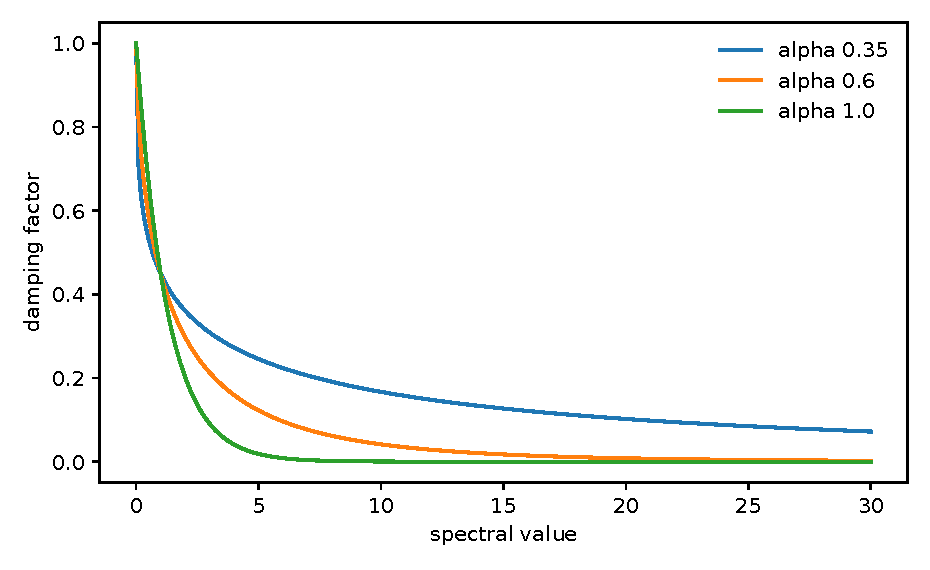
\includegraphics[width=0.72\textwidth]{fractional_damping.pdf}
\caption{Fractional damping of spectral packets. Smaller powers compress the separation among high frequencies while the packet eigenvectors remain unchanged.}
\label{fig:fractional_damping}
\end{figure}

\section{Green operators and discrete refinement}\label{sec:green}

Consider the Dirichlet operator
\[
L=-\frac{\dd^2}{\dd x^2}
\]
on \((0,1)\). Its Green kernel is
\[
G(x,y)=\min\{x,y\}-xy.
\]
For a continuous source \(f\), the solution of
\[
-u''=f,
\qquad
u(0)=u(1)=0
\]
is
\[
u(x)=\int_0^1G(x,y)f(y)\dd y.
\]

Let \(h=1/(n+1)\), let \(x_i=ih\), and define
\[
L_h
=
\frac1{h^2}
\begin{pmatrix}
2&-1&&\\
-1&2&\ddots&\\
&\ddots&\ddots&-1\\
&&-1&2
\end{pmatrix}.
\]

\begin{theorem}[Exact discrete Green reconstruction]\label{thm:discrete_green_reconstruction}
For \(1\leq i,j\leq n\),
\[
\boxed{
\frac1h(L_h^{-1})_{ij}
=
G(x_i,x_j).
}
\]
Thus the inverse finite difference matrix samples the continuum Green kernel exactly after the natural quadrature scaling.
\end{theorem}

\begin{proof}
For \(i\leq j\), the inverse of the unscaled tridiagonal matrix has entry
\[
\frac{i(n+1-j)}{n+1}.
\]
Multiplication by \(h^2\) gives
\[
(L_h^{-1})_{ij}
=
\frac{i(n+1-j)}{(n+1)^3}.
\]
Hence
\[
\frac1h(L_h^{-1})_{ij}
=
\frac{i}{n+1}
\left(1-\frac{j}{n+1}\right)
=x_i(1-x_j)
=G(x_i,x_j).
\]
The case \(j\leq i\) follows by symmetry.
\end{proof}

\begin{proposition}[Discrete Dirichlet spectrum]\label{prop:discrete_dirichlet_spectrum}
The eigenvectors of \(L_h\) are the sine modes
\[
v_k(i)=\sin(k\pi ih),
\qquad
1\leq k\leq n,
\]
with eigenvalues
\[
\boxed{
\lambda_{k,h}
=
\frac4{h^2}
\sin^2\left(\frac{k\pi h}{2}\right).
}
\]
\end{proposition}

\begin{proof}
Insert the sine addition formulas into the three point difference operator. The boundary values vanish because \(v_k(0)=v_k(n+1)=0\).
\end{proof}

\begin{theorem}[Second order low mode dispersion]\label{thm:low_mode_dispersion}
For every \(1\leq k\leq n\),
\[
\boxed{
0
\leq
(k\pi)^2-\lambda_{k,h}
\leq
\frac{(k\pi)^4}{12}h^2.
}
\]
\end{theorem}

\begin{proof}
Set \(x=k\pi h/2\), so \(0<x<\pi/2\). Since \(\sin x\leq x\), the left inequality follows. The elementary bound
\[
\sin x\geq x-\frac{x^3}{6}
\]
gives
\[
\sin^2x\geq x^2-\frac{x^4}{3}.
\]
Therefore
\[
\frac4{h^2}(x^2-\sin^2x)
\leq
\frac4{3h^2}x^4
=
\frac{(k\pi)^4}{12}h^2.
\]
\end{proof}

\begin{corollary}[Fractional low mode dispersion]\label{cor:fractional_low_mode_dispersion}
Let \(0<\alpha\leq1\). Then
\[
0
\leq
(k\pi)^{2\alpha}-\lambda_{k,h}^\alpha
\leq
\frac{\alpha(4k^2)^{\alpha-1}(k\pi)^4}{12}h^2.
\]
For every \(t\geq0\),
\[
\abs{
\e^{-t\lambda_{k,h}^\alpha}
-
\e^{-t(k\pi)^{2\alpha}}
}
\leq
\frac{t\alpha(4k^2)^{\alpha-1}(k\pi)^4}{12}h^2.
\]
\end{corollary}

\begin{proof}
The chord bound \(\sin x\geq2x/\pi\) on \([0,\pi/2]\) gives \(\lambda_{k,h}\geq4k^2\). Since \(x\mapsto x^\alpha\) is increasing and has decreasing derivative,
\[
(k\pi)^{2\alpha}-\lambda_{k,h}^\alpha
\leq
\alpha\lambda_{k,h}^{\alpha-1}
\bigl((k\pi)^2-\lambda_{k,h}\bigr).
\]
Use \cref{thm:low_mode_dispersion} and the lower bound for \(\lambda_{k,h}\). The exponential estimate follows from
\[
\abs{\e^{-ta}-\e^{-tb}}
\leq t\abs{a-b}
\]
for nonnegative \(a\) and \(b\).
\end{proof}

\begin{figure}
\centering
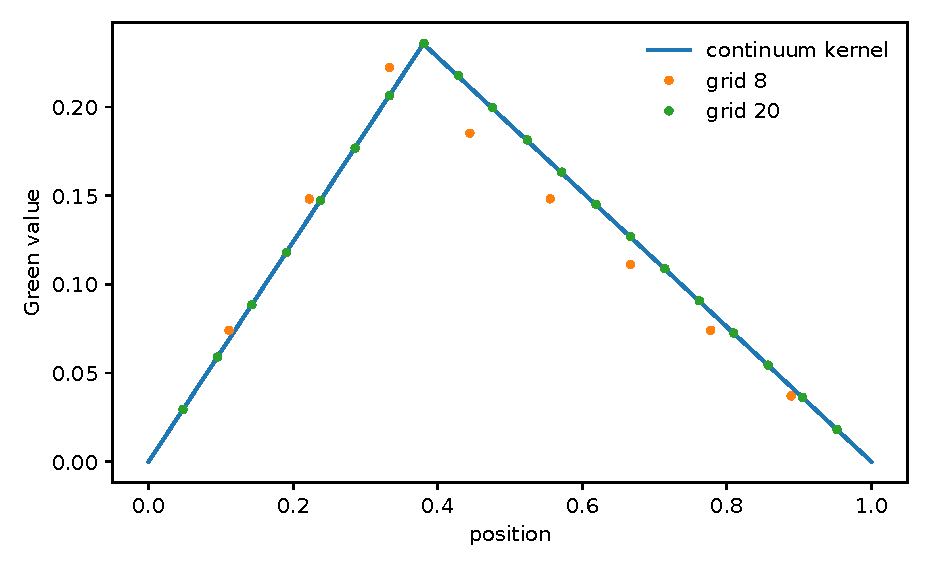
\includegraphics[width=0.72\textwidth]{green_kernel.pdf}
\caption{The Dirichlet Green kernel and its exact values on the finite difference grid. The matrix inverse reproduces the sampled kernel after one factor of the grid spacing.}
\label{fig:green_kernel}
\end{figure}

\begin{remark}
The exact identity in \cref{thm:discrete_green_reconstruction} is special to the one dimensional uniform Dirichlet grid. The spectral estimates illustrate how the abstract fractional refinement theory can be paired with a concrete discretization error.
\end{remark}

\section{Finite state Feynman Kac transfer}\label{sec:feynman_kac}

Let \(Q\) be a finite Markov generator in the column convention of \cref{sec:markov}. Its backward generator on functions is \(Q^T\). Let \(V=\diag(V_1,\ldots,V_n)\) with \(V_i\geq0\).

\begin{theorem}[Finite state Feynman Kac formula]\label{thm:finite_feynman_kac}
Let \((X_t)_{t\geq0}\) be the continuous time Markov chain with generator \(Q\). For every function \(f\in\RR^n\),
\[
\boxed{
\left(\e^{t(Q^T-V)}f\right)_i
=
\EE_i\left[
\exp\left(-\int_0^tV_{X_s}\dd s\right)
f(X_t)
\right].
}
\]
\end{theorem}

\begin{proof}
Let the right side be \(u_i(t)\). A first jump decomposition over a short interval gives
\[
\dot u(t)=(Q^T-V)u(t),
\qquad
u(0)=f.
\]
The finite linear initial value problem has the unique solution \(u(t)=\e^{t(Q^T-V)}f\).
\end{proof}

\begin{proposition}[Trotter path slicing]\label{prop:trotter_path_slicing}
For every \(t\geq0\),
\[
\boxed{
\e^{t(Q^T-V)}
=
\lim_{m\to\infty}
\left(
\e^{tQ^T/m}
\e^{-tV/m}
\right)^m
}
\]
in operator norm.
\end{proposition}

\begin{proof}
This is the Lie product formula for finite matrices. It follows by comparing the logarithm of one factor with \(t(Q^T-V)/m\) and using uniform boundedness of the finite products.
\end{proof}

\begin{theorem}[Potential perturbation bound]\label{thm:feynman_kac_potential_bound}
Let \(V\) and \(W\) be nonnegative diagonal matrices. In the supremum norm,
\[
\boxed{
\norm{
\e^{t(Q^T-V)}
-
\e^{t(Q^T-W)}
}_{\infty\to\infty}
\leq
 t\norm{V-W}_{\infty\to\infty}.
}
\]
\end{theorem}

\begin{proof}
Both killed Markov semigroups are contractions in the supremum norm. Apply the Duhamel identity with generator defect \(W-V\).
\end{proof}

\begin{theorem}[Coarse Feynman Kac transfer]\label{thm:coarse_feynman_kac}
Assume \(CQ=\overline QC\), and let \(J=C^T\) lift a coarse function to the corresponding block constant fine function. Suppose the potential is block constant, so
\[
VJ=J\overline V.
\]
Then
\[
\boxed{
\e^{t(Q^T-V)}J
=
J\e^{t(\overline Q^T-\overline V)}
}
\]
for every \(t\geq0\).
\end{theorem}

\begin{proof}
Transpose the Markov intertwining relation to obtain
\[
Q^TJ=J\overline Q^T.
\]
Together with \(VJ=J\overline V\), this gives
\[
(Q^T-V)J=J(\overline Q^T-\overline V).
\]
The exponential intertwining follows from the power series.
\end{proof}

\begin{figure}
\centering
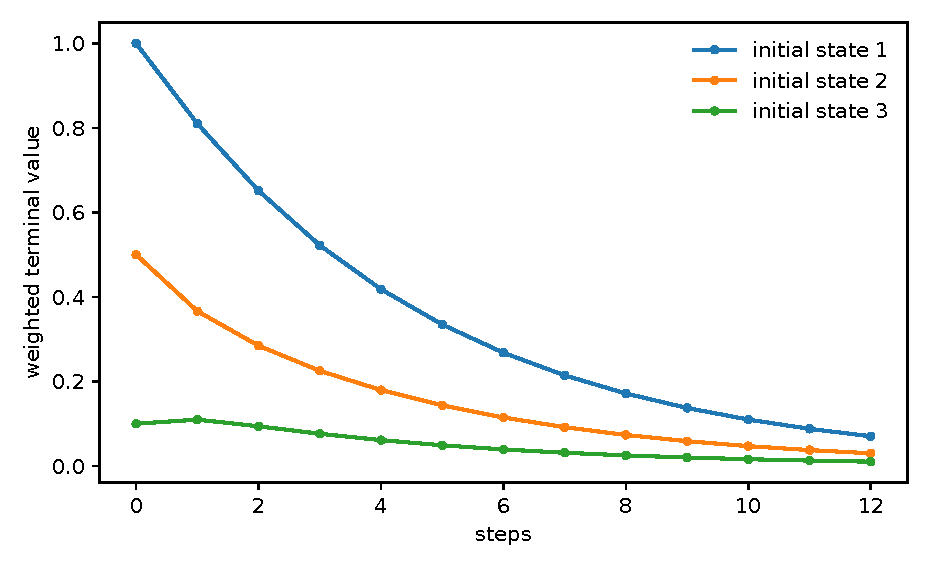
\includegraphics[width=0.72\textwidth]{feynman_kac.pdf}
\caption{A finite state path receives a multiplicative weight from the time spent in each potential packet. Block constant potentials preserve exact coarse transfer.}
\label{fig:feynman_kac}
\end{figure}

\section{Exact elimination and memory}\label{sec:memory}

Let a finite dimensional state space split as
\[
X=X_P\oplus X_Q.
\]
Let \(P:X\to X_P\) denote the coordinate projection onto the retained space.
Write the generator in block form
\[
A=
\begin{pmatrix}
A_{PP}&A_{PQ}\\
A_{QP}&A_{QQ}
\end{pmatrix}.
\]
The coordinates \(p(t)\in X_P\) are retained and \(q(t)\in X_Q\) are hidden.

\begin{theorem}[Schur Feshbach resolvent]\label{thm:schur_feshbach}
Whenever the displayed inverses exist,
\[
\boxed{
P(zI-A)^{-1}P
=
\left(
 zI-A_{PP}
-A_{PQ}(zI-A_{QQ})^{-1}A_{QP}
\right)^{-1}.
}
\]
The matrix valued function
\[
\Sigma(z)
=
A_{PQ}(zI-A_{QQ})^{-1}A_{QP}
\]
is the self energy of the retained coordinates.
\end{theorem}

\begin{proof}
Solve the hidden block equation
\[
(zI-A_{QQ})q=A_{QP}p
\]
for \(q\), substitute it into the retained block equation, and invert the resulting Schur complement. This is the finite dimensional Feshbach formula \cite{Feshbach1958}.
\end{proof}

\begin{theorem}[Exact memory equation]\label{thm:exact_memory_equation}
The retained coordinate of the system
\[
\frac{\dd}{\dd t}
\begin{pmatrix}p\\q\end{pmatrix}
=A
\begin{pmatrix}p\\q\end{pmatrix}
\]
satisfies
\[
\boxed{
\dot p(t)
=
A_{PP}p(t)
+A_{PQ}\e^{tA_{QQ}}q(0)
+
\int_0^t
\Kcal(t-s)p(s)\dd s,
}
\]
where
\[
\boxed{
\Kcal(t)
=
A_{PQ}\e^{tA_{QQ}}A_{QP}.
}
\]
For \(\operatorname{Re}z\) sufficiently large,
\[
\widehat\Kcal(z)
=
\int_0^\infty\e^{-zt}\Kcal(t)\dd t
=
\Sigma(z).
\]
\end{theorem}

\begin{proof}
Variation of constants in the hidden equation gives
\[
q(t)=\e^{tA_{QQ}}q(0)
+
\int_0^t\e^{(t-s)A_{QQ}}A_{QP}p(s)\dd s.
\]
Substitute this expression into the retained equation. The Laplace transform follows from
\[
\int_0^\infty\e^{-zt}\e^{tA_{QQ}}\dd t
=(zI-A_{QQ})^{-1}.
\]
\end{proof}

\begin{theorem}[Criterion for an exact local closure]\label{thm:exact_local_closure}
Let \(d_Q=\dim X_Q\). The following statements are equivalent.
\begin{enumerate}
\item There is an operator \(B\) on \(X_P\) such that, for every initial retained state and \(q(0)=0\),
\[
p(t)=\e^{tB}p(0)
\]
for all \(t\geq0\).
\item For all sufficiently large \(z\),
\[
P(zI-A)^{-1}P=(zI-B)^{-1}.
\]
\item \(B=A_{PP}\) and \(\Sigma(z)\equiv0\).
\item
\[
A_{PQ}A_{QQ}^kA_{QP}=0
\]
for \(k=0,1,\ldots,d_Q-1\).
\end{enumerate}
\end{theorem}

\begin{proof}
The Laplace transform of the retained evolution proves the equivalence of the first two statements. By \cref{thm:schur_feshbach}, equality of the two resolvents implies
\[
zI-A_{PP}-\Sigma(z)=zI-B.
\]
Letting \(z\) tend to infinity gives \(B=A_{PP}\), and then \(\Sigma(z)=0\). The converse is immediate.

For large \(z\),
\[
\Sigma(z)
=
\sum_{k=0}^\infty
z^{-k-1}
A_{PQ}A_{QQ}^kA_{QP}.
\]
Thus \(\Sigma\equiv0\) if and only if every coefficient vanishes. By the Cayley Hamilton theorem, the powers \(A_{QQ}^k\) for \(k\geq d_Q\) are linear combinations of the first \(d_Q\) powers. It is therefore enough to test the stated finite list.
\end{proof}


\begin{example}[One hidden mode]\label{ex:one_hidden_mode}
Consider
\[
A=
\begin{pmatrix}
-a&c\\
d&-b
\end{pmatrix},
\qquad
a,b>0,
\]
and retain the first coordinate. The memory kernel and self energy are
\[
\Kcal(t)=cd\e^{-bt},
\qquad
\Sigma(z)=\frac{cd}{z+b}.
\]
The retained coordinate has an exact time local closure for every retained initial value precisely when \(cd=0\). When \(cd\neq0\), one auxiliary scalar state realizes the memory exactly.
\end{example}

\begin{definition}[Finite auxiliary realization]\label{def:finite_auxiliary_realization}
A memory kernel \(\Kcal\) has a finite auxiliary realization if there are finite dimensional matrices \(B,D,C\) such that
\[
\Kcal(t)=B\e^{tD}C.
\]
The enlarged local system is
\[
\dot p=A_{PP}p+By,
\qquad
\dot y=Dy+Cp.
\]
\end{definition}

\begin{theorem}[Rational memory realization]\label{thm:rational_memory_realization}
A matrix valued memory transform has a finite auxiliary realization if and only if it is a strictly proper rational matrix function. More precisely,
\[
\boxed{
\widehat\Kcal(z)=B(zI-D)^{-1}C
}
\]
if and only if
\[
\boxed{
\Kcal(t)=B\e^{tD}C.
}
\]
\end{theorem}

\begin{proof}
The forward implication follows by taking the Laplace transform. The resulting matrix is rational and tends to zero as \(z\) tends to infinity.

Conversely, decompose every entry of a strictly proper rational matrix into partial fractions. A term
\[
\frac{c}{(z-\lambda)^r}
\]
is an entry of the resolvent of an \(r\) by \(r\) Jordan block with eigenvalue \(\lambda\). Taking a direct sum of these blocks and choosing the input and output maps entry by entry gives matrices \(B,D,C\) with the required resolvent. Inverse Laplace transformation gives the time domain formula.
\end{proof}

\begin{corollary}[Exponential sum memory]\label{cor:exponential_sum_memory}
If
\[
\Kcal(t)=\sum_{j=1}^{m}B_j\e^{\lambda_jt}C_j,
\]
then \(\Kcal\) has a finite auxiliary realization with one auxiliary block for each exponential. Repeated poles produce polynomial factors in \(t\) and are realized by Jordan blocks.
\end{corollary}

\begin{proof}
Use a block diagonal matrix \(D\) whose blocks are the scalars \(\lambda_j\), or the required Jordan blocks when poles repeat. Assemble the matrices \(B_j\) and \(C_j\) into the output and input maps.
\end{proof}

\begin{theorem}[Stability of memory compression]\label{thm:memory_compression_stability}
Let \(x\) and \(\widetilde x\) solve
\[
\dot x(t)
=Ax(t)+\int_0^t\Kcal(t-s)x(s)\dd s+f(t)
\]
and
\[
\dot{\widetilde x}(t)
=A\widetilde x(t)
+\int_0^t\widetilde\Kcal(t-s)\widetilde x(s)\dd s
+f(t)
\]
with the same initial value. Fix \(T>0\), and assume
\[
\sup_{0\leq t\leq T}\norm{\widetilde x(t)}\leq M.
\]
Set
\[
a=\norm A,
\qquad
k=\norm{\Kcal}_{L^1(0,T)},
\qquad
\delta=\norm{\Kcal-\widetilde\Kcal}_{L^1(0,T)}.
\]
Then
\[
\boxed{
\sup_{0\leq t\leq T}
\norm{x(t)-\widetilde x(t)}
\leq
MT\delta\e^{(a+k)T}.
}
\]
\end{theorem}

\begin{proof}
Let \(e=x-\widetilde x\). Integrating the difference equation and changing the order of integration gives
\[
\norm{e(t)}
\leq
(a+k)\int_0^t\norm{e(r)}\dd r
+Mt\delta.
\]
Since \(t\leq T\), Gronwall's inequality gives
\[
\norm{e(t)}
\leq
MT\delta\e^{(a+k)t}.
\]
Take the supremum over \([0,T]\).
\end{proof}

\begin{figure}
\centering
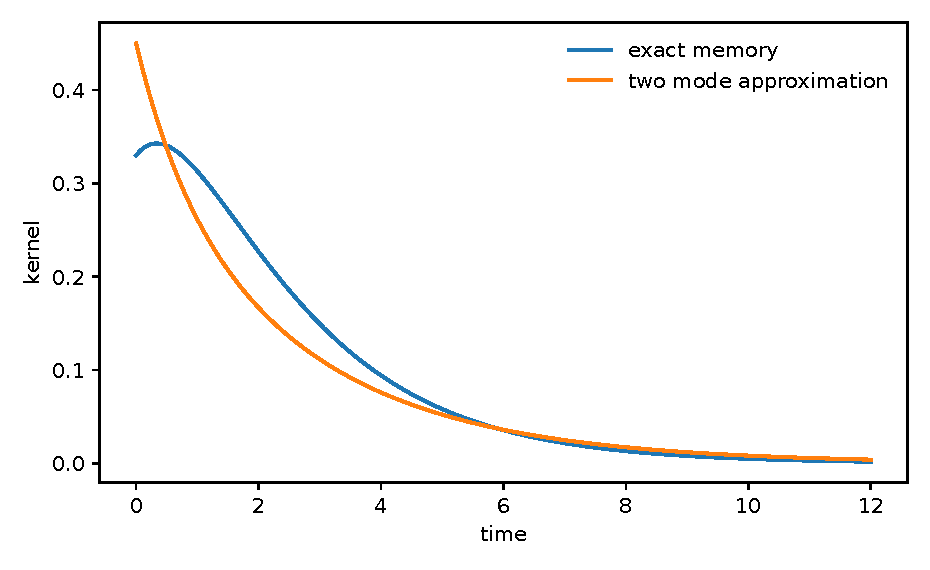
\includegraphics[width=0.74\textwidth]{memory_kernel.pdf}
\caption{Hidden coordinates produce a memory kernel on the retained state. A finite auxiliary system replaces the convolution exactly when the memory transform is strictly proper and rational.}
\label{fig:memory_kernel}
\end{figure}

\begin{remark}
A small kernel error is not by itself enough for a useful approximation on arbitrarily long time intervals. The bound in \cref{thm:memory_compression_stability} is finite horizon and depends on a bound for the approximate trajectory. Stability of the auxiliary realization remains a separate requirement.
\end{remark}

\section{Survival and hazard semigroups}\label{sec:survival}

Let \(A\in\RR^{n\times n}\) be a transient Markov subgenerator. Its off diagonal entries are nonnegative, its column sums are nonpositive, and every eigenvalue has negative real part. Let \(p_0\) be an initial transient distribution. Define
\[
p(t)=\e^{tA}p_0.
\]
The absorption rate row is
\[
a^T=-\one^TA.
\]

\begin{theorem}[Survival, density, and hazard]\label{thm:survival_density_hazard}
The survival function, absorption density, and hazard are
\[
\boxed{
S(t)=\one^T\e^{tA}p_0,
}
\]
\[
\boxed{
f(t)=a^T\e^{tA}p_0=-S'(t),
}
\]
and
\[
\boxed{
h(t)=\frac{f(t)}{S(t)}
}
\]
whenever \(S(t)>0\).
\end{theorem}

\begin{proof}
The total transient mass is \(S(t)\). Differentiate it:
\[
S'(t)=\one^TA\e^{tA}p_0=-a^T\e^{tA}p_0.
\]
Since all transient mass is eventually absorbed, \(-S'\) is the absorption density. The hazard is its conditional rate relative to the surviving mass.
\end{proof}

\begin{theorem}[Laplace transform and moments]\label{thm:survival_laplace_moments}
For \(\operatorname{Re}s\geq0\),
\[
\boxed{
\EE[\e^{-s\tau}]
=
a^T(sI-A)^{-1}p_0.
}
\]
For every integer \(m\geq1\),
\[
\boxed{
\EE[\tau^m]
=
m!\one^T(-A)^{-m}p_0.
}
\]
\end{theorem}

\begin{proof}
The Laplace transform follows from
\[
\int_0^\infty\e^{-st}f(t)\dd t
=
a^T(sI-A)^{-1}p_0.
\]
Integration by parts gives
\[
\EE[\tau^m]
=m\int_0^\infty t^{m-1}S(t)\dd t.
\]
For a stable matrix \(A\),
\[
\int_0^\infty t^{m-1}\e^{tA}\dd t
=(m-1)!(-A)^{-m}.
\]
Substitution proves the moment formula.
\end{proof}

\begin{corollary}[Phase type rationality]\label{cor:phase_type_rationality}
The Laplace transform of every finite phase type distribution is rational. If \(A\) is diagonalizable, then \(S(t)\) and \(f(t)\) are finite linear combinations of exponential functions. Jordan blocks add polynomial factors in \(t\).
\end{corollary}

\begin{proof}
The resolvent \((sI-A)^{-1}\) is rational. The time domain statement follows from the Jordan form of \(A\).
\end{proof}

\begin{corollary}[One phase model]\label{cor:one_phase_model}
If \(A=(-\lambda)\) and \(p_0=1\), then
\[
S(t)=\e^{-\lambda t},
\qquad
f(t)=\lambda\e^{-\lambda t},
\qquad
h(t)=\lambda.
\]
\end{corollary}

\begin{proof}
Insert the scalar generator into \cref{thm:survival_density_hazard}.
\end{proof}


\begin{example}[Two sequential phases]\label{ex:two_phase_survival}
Let
\[
A=
\begin{pmatrix}
-\lambda&0\\
\lambda&-\mu
\end{pmatrix},
\qquad
p_0=
\begin{pmatrix}1\\0\end{pmatrix},
\]
where \(\lambda\neq\mu\) are positive. The first phase moves to the second at rate \(\lambda\), and the second is absorbed at rate \(\mu\). Direct calculation gives
\[
S(t)=
\frac{\mu\e^{-\lambda t}-\lambda\e^{-\mu t}}{\mu-\lambda},
\]
\[
f(t)=
\frac{\lambda\mu}{\mu-\lambda}
\left(\e^{-\lambda t}-\e^{-\mu t}\right).
\]
The ratio \(f(t)/S(t)\) is generally not constant. A time local Markov model on two transient phases can therefore produce a nonconstant hazard after the phase coordinate is hidden.
\end{example}

\begin{figure}
\centering
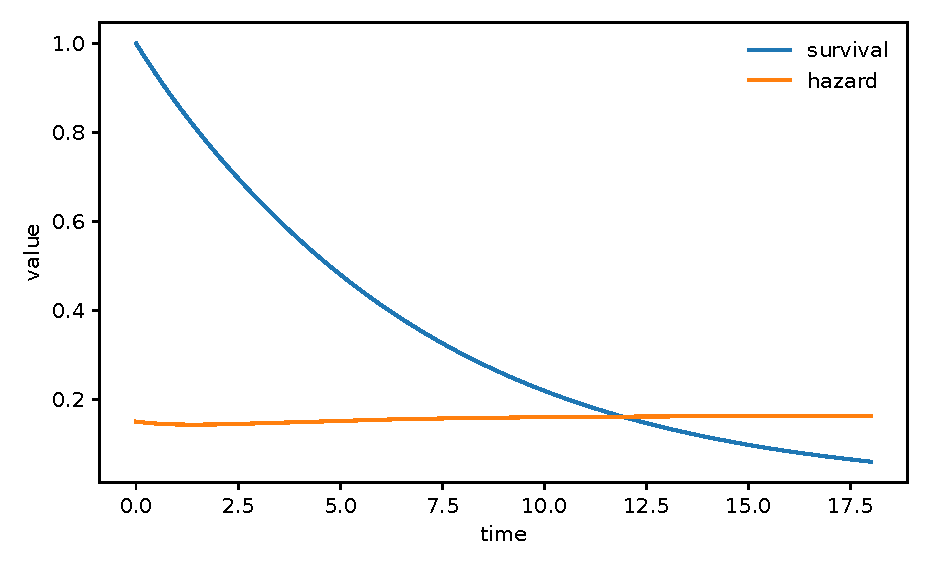
\includegraphics[width=0.72\textwidth]{survival_hazard.pdf}
\caption{Survival and hazard generated by a finite transient semigroup. Several hidden phases can produce a nonconstant hazard even though the enlarged model is time local.}
\label{fig:survival_hazard}
\end{figure}

\section{Finite illustrations and verification scope}\label{sec:finite_illustrations}

The figures in this article are generated from finite examples that mirror the exact formulas. They serve three purposes. They show the scale of the quantities in the estimates, they expose the difference between exact and defective refinement, and they provide reproducible tests of the implementations. They do not replace the proofs.

\begin{table}
\centering
\caption{Representative identities used in the finite verification suite.}
\label{tab:verification_identities}
\begin{tabular}{>{\raggedright\arraybackslash}p{0.24\textwidth}>{\raggedright\arraybackslash}p{0.64\textwidth}}
\toprule
Mechanism & Verified identity \\
\midrule
Packet semigroup & Block convolution and time ordered path reconstruction \\
Refinement & Duhamel, resolvent, and several level telescoping identities \\
Markov aggregation & Aggregate rate criterion and exact coarse evolution \\
Bayesian aggregation & Sufficiency, information loss, and filter defect bounds \\
Fractional powers & Spectral formulas, exact naturality, and gap dependent defect bound \\
Green operator & Exact sampled kernel and second order eigenvalue error \\
Feynman Kac & Matrix exponential against finite path expectations \\
Memory & Schur complement, kernel transform, and auxiliary realization \\
Survival & Density, Laplace transform, and moment identities \\
\bottomrule
\end{tabular}
\end{table}

The machine checks use exact arithmetic when possible and high precision floating point arithmetic otherwise. Negative controls deliberately break intertwining, lumpability, sufficiency, or support conditions. The complete scripts and generated records accompany the source package.

\section{Limits and further questions}\label{sec:limits}

The results leave several distinct problems open.

First, exact projective compatibility gives a semigroup on the projective limit, but approximate compatibility alone does not identify a limiting generator. A stronger continuum theorem would require a topology, a dense compatible core, stability of the resolvents, and a convergence principle such as Trotter Kato approximation.

Second, finite Bayesian sufficiency is completely characterized for ordinary block aggregation. Approximate sufficiency over continuous state spaces requires a choice of statistical metric and regularity of the conditional likelihoods. The exact information loss formula suggests natural bounds, but it does not by itself identify a minimal coarse statistic.

Third, the fractional defect theorem uses positivity, self adjointness, and a spectral gap. Sectorial generators admit fractional powers through contour and resolvent formulas, but a comparable refinement estimate must account for sectorial constants and possible spectral behavior near zero.

Fourth, rational memory has a finite auxiliary realization, but minimal dimension and numerically stable realization are separate questions. Balanced truncation, Hankel singular values, and positivity constraints may give sharper compression theorems for particular classes of kernels.

Finally, the finite Green and Feynman Kac models are exact within their declared settings. Extension to rough coefficients, unbounded generators, infinite state chains, and nonlinear filtering requires additional domain and compactness arguments.

\section{Conclusion}\label{sec:conclusion}

Packet decomposition, refinement, and elimination describe three different views of an evolution. Packet blocks resolve where mass or amplitude travels. Refinement defects measure what a coarse model fails to preserve. Elimination records hidden dynamics as memory. The exact identities developed here show how these views fit together.

The packet semigroup law and path expansion resolve bounded evolution into transfers. Duhamel and resolvent formulas propagate a generator defect to the whole functional calculus. Markov lumping, conditional expectation, and Bayesian sufficiency give three precise forms of probabilistic coarse graining. Fractional powers inherit exact refinement and admit a quantitative gap dependent bound. Green operators and Feynman Kac weights provide spatial and path realizations. Schur elimination then identifies the exact memory kernel, while rational realization explains when that memory can be returned to a finite local system.

\section*{Disclosure concerning language model assistance}

An OpenAI language model was used as a drafting and organizational aid. It suggested formulations and proof approaches for the projective limit discussion in \cref{sec:refinement}, the finite Bayesian sufficiency and information loss results in \cref{sec:bayes,sec:filtering}, the fractional defect estimate in \cref{sec:fractional}, and the rational memory and compression results in \cref{sec:memory}. The author accepts full responsibility for the mathematical content and for independent verification of every statement, computation, and citation. The model is not an author.

\bibliographystyle{aomalpha}
\bibliography{PSC_Paper_VI_Annals_Human_Edition}

\end{document}
